% THIS IS SIGPROC-SP.TEX - VERSION 3.0
% WORKS WITH V3.1SP OF ACM_PROC_ARTICLE-SP.CLS
% JUNE 2007
%
% It is an example file showing how to use the 'acm_proc_article-sp.cls' V3.1SP
% LaTeX2e document class file for Conference Proceedings submissions.
% ----------------------------------------------------------------------------------------------------------------
% This .tex file (and associated .cls V3.1SP) *DOES NOT* produce:
%       1) The Permission Statement
%       2) The Conference (location) Info information
%       3) The Copyright Line with ACM data
%       4) Page numbering
% ---------------------------------------------------------------------------------------------------------------
% It is an example which *does* use the .bib file (from which the .bbl file
% is produced).
% REMEMBER HOWEVER: After having produced the .bbl file,
% and prior to final submission,
% you need to 'insert'  your .bbl file into your source .tex file so as to provide
% ONE 'self-contained' source file.
%
% Questions regarding SIGS should be sent to
% Adrienne Griscti ---> griscti@acm.org
%
% Questions/suggestions regarding the guidelines, .tex and .cls files, etc. to
% Gerald Murray ---> murray@acm.org
%
% For tracking purposes - this is V3.0SP - JUNE 2007

\documentclass{sig-alternate}
%\usepackage{latex8}
\usepackage{times}
\usepackage{graphicx}
\usepackage{epsf}
\usepackage{verbatim}
\usepackage{psfig}
\usepackage{cite}
\usepackage{url}
\usepackage{color}
\usepackage{alltt}

\usepackage{longtable,lscape}
\usepackage{slashbox,multirow}
\usepackage{colortbl}
\usepackage{mathrsfs}

\newcommand{\Add}{\CodeIn{add}}
\newcommand{\AVTree}{\CodeIn{AVTree}}
\newcommand{\Assignment}[3]{$\langle$ \Object{#1}, \Object{#2}, \Object{#3} $\rangle$}
\newcommand{\BinaryTreeRemove}{\CodeIn{BinaryTree\_remove}}
\newcommand{\BinaryTree}{\CodeIn{BinaryTree}}
\newcommand{\Caption}{\caption}
\newcommand{\Char}[1]{`#1'}
\newcommand{\CheckRep}{\CodeIn{checkRep}}
\newcommand{\ClassC}{\CodeIn{C}}
\newcommand{\CodeIn}[1]{{\small\texttt{#1}}}
\newcommand{\CodeOutSize}{\scriptsize}
\newcommand{\Comment}[1]{}
\newcommand{\Ensures}{\CodeIn{ensures}}
\newcommand{\ExtractMax}{\CodeIn{extractMax}}
\newcommand{\FAL}{field-ordering}
\newcommand{\FALs}{field-orderings}
\newcommand{\Fact}{observation}
\newcommand{\Get}{\CodeIn{get}}
\newcommand{\HashSet}{\CodeIn{HashSet}}
\newcommand{\HeapArray}{\CodeIn{HeapArray}}
\newcommand{\Intro}[1]{\emph{#1}}
\newcommand{\Invariant}{\CodeIn{invariant}}
\newcommand{\JUC}{\CodeIn{java.\-util.\-Collections}}
\newcommand{\JUS}{\CodeIn{java.\-util.\-Set}}
\newcommand{\JUTM}{\CodeIn{java.\-util.\-TreeMap}}
\newcommand{\JUTS}{\CodeIn{java.\-util.\-TreeSet}}
\newcommand{\JUV}{\CodeIn{java.\-util.\-Vector}}
\newcommand{\JMLPlusJUnit}{JML+JUnit}
\newcommand{\Korat}{Korat}
\newcommand{\Left}{\CodeIn{left}}
\newcommand{\Lookup}{\CodeIn{lookup}}
\newcommand{\MethM}{\CodeIn{m}}
\newcommand{\Node}[1]{\CodeIn{N}$_#1$}
\newcommand{\Null}{\CodeIn{null}}
\newcommand{\Object}[1]{\CodeIn{o}\ensuremath{_#1}}
\newcommand{\PostM}{\MethM$_{post}$}
\newcommand{\PreM}{\MethM$_{pre}$}
\newcommand{\Put}{\CodeIn{put}}
\newcommand{\Remove}{\CodeIn{remove}}
\newcommand{\RepOk}{\CodeIn{repOk}}
\newcommand{\Requires}{\CodeIn{requires}}
\newcommand{\Reverse}{\CodeIn{reverse}}
\newcommand{\Right}{\CodeIn{right}}
\newcommand{\Root}{\CodeIn{root}}
\newcommand{\Set}{\CodeIn{set}}
\newcommand{\State}[1]{2^{#1}}
\newcommand{\TestEra}{TestEra}
\newcommand{\TreeMap}{\CodeIn{TreeMap}}

\newenvironment{CodeOut}{\begin{scriptsize}}{\end{scriptsize}}
\newenvironment{SmallOut}{\begin{small}}{\end{small}}

\newcommand{\pairwiseEquals}{PairwiseEquals}
\newcommand{\monitorEquals}{MonitorEquals}
%\newcommand{\monitorWField}{WholeStateW}
\newcommand{\traverseField}{WholeState}
\newcommand{\monitorSMSeq}{ModifyingSeq}
\newcommand{\monitorSeq}{WholeSeq}

\newcommand{\IntStack}{\CodeIn{IntStack}}
\newcommand{\UBStack}{\CodeIn{UBStack}}
\newcommand{\BSet}{\CodeIn{BSet}}
\newcommand{\BBag}{\CodeIn{BBag}}
\newcommand{\ShoppingCart}{\CodeIn{ShoppingCart}}
\newcommand{\BankAccount}{\CodeIn{BankAccount}}
\newcommand{\BinarySearchTree}{\CodeIn{BinarySearchTree}}
\newcommand{\LinkedList}{\CodeIn{LinkedList}}

\newcommand{\Book}{\CodeIn{Book}}
\newcommand{\Library}{\CodeIn{Library}}

\newcommand{\Jtest}{Jtest}
\newcommand{\JCrasher}{JCrasher}
\newcommand{\Daikon}{Daikon}
\newcommand{\JUnit}{JUnit}

\newcommand{\trie}{trie}

\newcommand{\Perl}{Perl}


\newcommand{\SubjectCount}{11}
\newcommand{\DSSubjectCount}{two}

\newcommand{\Equals}{\CodeIn{equals}}
\newcommand{\Pairwise}{PairwiseEquals}
\newcommand{\Subgraph}{MonitorEquals}
\newcommand{\Concrete}{WholeState}
\newcommand{\ModSeq}{ModifyingSeq}
\newcommand{\Seq}{WholeSeq}
\newcommand{\Aeq}{equality}

\newcommand{\Meaning}[1]{\ensuremath{[\![}#1\ensuremath{]\!]}}
\newcommand{\Pair}[2]{\ensuremath{\langle #1, #2 \rangle}}
\newcommand{\Triple}[3]{\ensuremath{\langle #1, #2, #3 \rangle}}
\newcommand{\SetSuch}[2]{\ensuremath{\{ #1 | #2 \}}}

\newcommand{\Equiv}[2]{\ensuremath{#1 \EquivSTRel{} #2}}
\newcommand{\EquivME}{\Equiv}
\newcommand{\EquivST}{\Equiv}
\newcommand{\EquivSTRel}{\ensuremath{\cong}}
\newcommand{\Redundant}[2]{\ensuremath{#1 \lhd #2}}
\newcommand{\VB}{\ensuremath{\mid}}
\newcommand{\MES}{method-entry state}

\newcommand{\Small}[1]{{\small{#1}}}

\newcommand{\CenterCell}[1]{\multicolumn{1}{c|}{#1}}

\begin{document}

\title{An Empirical Study of Retrofitting Legacy Unit Tests for Parameterized Unit Testing}

%\numberofauthors{5} 
\author{Madhuri R. Marri$^1$, Suresh Thummalapenta$^1$, Tao Xie$^1$, Nikolai Tillmann$^2$, Jonathan de Halleux$^2$\\
\small{$^1$Department of Computer Science, North Carolina State University, Raleigh, NC}\\
\small{$^2$Microsoft Research, One Microsoft Way, Redmond, WA}\\
\small{$^1$\{mrmarri, sthumma, txie\}@ncsu.edu, $^2$\{nikolait, jhalleux\}@microsoft.com}\\}
\maketitle
%\begin{abstract}
%Owing to the significance of unit testing in the software development life cycle, unit testing has been widely adopted by software industry to ensure high-quality software. It is labor-intensive to write high-covering tests to ensure the software quality and therefore calls for automation. One such automatic testing technique to achieve high-covering tests is to write Parameterized Unit Tests (PUTs) and use them in combination with a test generation tool that accepts these PUTs. PUTs are a generalized form of conventional unit tests that accept parameters and where programmers can describe the expected behavior or specifications in a generic manner. An automatic test generation tool such as Pex from Microsoft Research accepts these PUTs and generates a set of conventional unit tests to achieve a high code coverage. We conduct an empirical study to investigate the utility of PUTs to generate high-covering conventional unit tests. In our empirical study, we use an open source C\# project, called NUnit, to study the benefits of PUTs over conventional unit tests. In this paper, we present our empirical study carried out in two phases: test generalization (transforming existing manually written conventional unit tests to PUTs) and writing new PUTs (to cover the code portions under test that are not covered by the transformed PUTs). In our study, we found that test generalization increased the average block coverage by $9.68$\% with a maximum increase of $45.26\%$ for one class under test. Writing new PUTs resulted in a total increase of $17.41$\% on an average. We also found that testing with PUTs detected $7$ new defects that were not detected by the existing conventional unit tests.
%\end{abstract}
%\vspace*{-4ex}
%----------------------------------------------------------------------------------------------
\section{Introduction}
\label{sec:introduction}

Since the inception of computer science, many programming languages (\emph{e.g.}, Cobol, Fortran, or Java) have been introduced to serve specific requirements\footnote{\url{http://hopl.murdoch.edu.au}}. For example, Cobol is introduced specifically for developing business applications. In general, software companies or open source organizations often release their applications in different languages to survive in competing markets and to address various business requirements such as platform independence. An empirical study~\citep{jones1998estimating} shows that nearly one third applications have multiple versions in different languages. A natural way to implement an application in a different language is to translate from an existing application. For example, Lucene.Net was translated from Java Lucene according to its website\footnote{\url{http://lucene.apache.org/lucene.net/}}. As another example, the NeoDatis object database was also translated form Java to C\# according to its website\footnote{\url{http://wiki.neodatis.org/}}. During translation, one primary goal is to ensure that both applications exhibit the same behavior.

As existing applications typically use API libraries, it is essential to understand API mapping relations of one programming language, referred to as $L_1$, to another language, referred to as $L_2$, when translating applications from $L_1$ to $L_2$. Researchers~\citep{robillard2009makes,thomas2006api} pointed out that it is hard to use API elements, and our previous work~\citep{zhong2010mining} shows that mapping relations between API elements of different languages can also be complicated. In some cases, programmers may fail to find an existing API element that has the same behavior in the other language. For example, Figures~\ref{fig:db4ojava} and \ref{fig:db40net} show two methods implemented in db4o\footnote{\url{http://www.db4o.com}} of its Java version and its C\# version, respectively. When translating the Java code shown in Figure~\ref{fig:db4ojava} to C\#, programmers of db4o may fail to find an existing C\# class that has the same behaviors with the \CodeIn{Byte\-Array\-Input\-Stream} class in Java, so they implement a C\# class with the same name to fix the behavioral difference. Behavioral differences of mapped API elements (\emph{i.e}., classes, methods, and fields of API libraries) may occur in many places. To reduce translation effort, programmers of db4o developed their own translation tool, called Sharpen\footnote{\url{http://developer.db4o.com/Blogs/News/tabid/171/entryid/653/Default.aspx}}, for translating db4o from Java to C\#. For API translation, Sharpen systematically replaces all API elements in Java with equivalent elements in C\# to ensure that translated C\# applications have the same behaviors with the original Java ones.

\begin{figure}[t]
\begin{CodeOut}%\vspace*{-2ex}
\begin{alltt}
01: private long readLong(ByteArrayInputStream is)\{
02:  ...
03:  l += ((long) (is.read())) << i;
04:  ...\}
\end{alltt}
\end{CodeOut}%\vspace*{-4ex}
\caption{A method in the Java version of db4o.}%\vspace*{-2ex}
\label{fig:db4ojava}
\begin{CodeOut}%\vspace*{-2ex}
\begin{alltt}
05: private long ReadLong(ByteArrayInputStream @is)\{
06:  ...
07:  l += ((long)(@is.Read())) << i;
08:  ...\}
\end{alltt}
\end{CodeOut}%\vspace*{-4ex}
\caption{A method in the C\# version of db4o.}%\vspace*{-4ex}
\label{fig:db40net}
\end{figure}

In practice, as pointed out by Keyvan Nayyeri\footnote{\url{http://dotnet.dzone.com/print/26587}}, one of the most common problems is that translated code does not return expected outputs, partially because behavioral differences of mapped API elements are not fully fixed. For example, when JLCA\footnote{JLCA is a Java-to-C\# translation tool developed by Microsoft. The website of JLCA is \url{http://msdn.microsoft.com/en-us/magazine/cc163422.aspx}} translates the \CodeIn{java.lang.String.indexOf(int)} method from Java to C\#, it generates a warning message: ``Method \CodeIn{java.lang.String. indexOf} was converted to \CodeIn{System.String.IndexOf}, which may throw an exception''. Still, the report does not describe where such an exception is thrown or how to deal with that exception. As programmers typically do not know where such behavioral differences occur, it is difficult for programmers to fix such differences in advance, and thus defects can be introduced in translated applications. To prevent those defects, it is desirable to detect behavioral differences between mapped API elements in different languages. However, existing approaches~\citep{orso1using,jin2010automated,jiang2009automatic,lindigaadebug2005} solve different problems, and cannot detect such differences effectively since these existing approaches require that both the versions under consideration belong to the same language. In our context, the versions under consideration belong to different languages, making these existing approaches inapplicable.


To address the preceding issue, we propose a novel approach, called TeMAPI (\textbf{Te}sting \textbf{Ma}pping relations of \textbf{API}s), that generates test cases to detect behavioral differences among API mapping relations automatically. In particular, TeMAPI accepts two inputs: a translation tool under analysis and a test-generation tool for generating test cases. Given a translation tool that translates applications from one language $L_1$ to the other language $L_2$, TeMAPI generates various test cases to detect behavioral differences among the API mapping relations by effectively leveraging the test-generation tool. TeMAPI next executes translated test cases to detect behavioral differences.

TeMAPI addresses four major technical challenges in effectively detecting behavioral differences. (1) It is challenging to directly extract API mapping relations from translation tools. The primary reason is that often translation tools either use different formats for specifying API mapping relations or do not explicitly describe these mapping relations. For example, Java2CSharp\footnote{Java2CSharp is a Java-to-C\# translation tool developed by ILOG (now IBM). The website of Java2CSharp is \url{http://j2cstranslator.sourceforge.net/}} uses mapping files, Sharpen hardcodes relations in source files, and closed source translation tools such as JLCA typically hide mapping relations in binary files. To address this issue and to be independent of the translation tool under analysis, TeMAPI analyzes translated code for extracting those relations. (2) Interfaces of two mapped API elements can be different, and one API element can be translated to multiple API elements. For example, JLCA translates the \CodeIn{java.net.DatagramSocket.receive(DatagramPacket)} method in Java as shown in Figure~\ref{fig:javacode} to multiple C\# elements as shown in Figure~\ref{fig:codeJLCA}.
To address this issue, TeMAPI uses a technique, called wrapper methods (Section~\ref{sec:approach:wrapper}), that abstracts interface differences among mapped API elements and provides a common interface to effectively apply test-generation tools. (3) Using a basic technique such as generating test cases with \CodeIn{null} values may not be significant in detecting behavioral differences among API mapping relations. Since we focus on object-oriented languages such as Java or C\# to detect behavioral differences, generated test cases need to exercise various object states, which can be achieved using method-call sequences. To address this issue, TeMAPI leverages two existing state-of-the-art test-generation techniques: random~\citep{pacheco2007feedback} and dynamic-symbolic-execution-based~\citep{koushik:cute, godefroid:dart, tillmann2008pex} ones. (4) API elements are typically quite large in size, and it is difficult to check all outputs, posing a test oracle barrier. To overcome the barrier, TeMAPI uses return values of wrapper methods or exceptions being thrown as test oracles. We describe more details of our approach to address these challenges in subsequent sections.

In this paper, although we present our approach for detecting behavioral differences among mapping relations of different languages, our approach is general and can be applied to other software engineering problems where an API needs to be replaced with another API without changing the behavior of an application (\emph{e.g.}, library upgrades~\citep{Kawrykow:2009} or migrating from one library to another library~\citep{nita2010using}).

This paper makes the following major contributions:

\begin{itemize}\vspace*{-1ex}
\item A novel approach, called TeMAPI, that automatically generates test cases to detect behavioral differences among API mapping relations. %\vspace*{-1.5ex}
\item A tool implemented for TeMAPI and four evaluations on five popular translation tools. Unlike untranslated code elements, behavioral differences introduce no compilation errors to be detected, and can lead to defects in translated applications silently. Our results show that existing translation tools can translate most lines from Java to C\#, although these tools typically cover a small set of API mapping relations. Our results also show the effectiveness of our approach in detecting behavioral differences of mapped API elements between different languages.
\item The first empirical comparison on behavioral differences of mapped API elements between the J2SE and .NET frameworks. As shown in Section~\ref{sec:evaluation}, the comparison reveals 8 behavioral differences between mapped API elements in existing translation tools. We analyze these findings, and conclude their implications that are valuable to vendors of translation tools for improving their tools, programmers who use translation tools for being aware of such differences in advance, and developers of API libraries for implementing more translatable APIs.
\end{itemize}\vspace*{-1ex}

The rest of this paper is organized as follows.
%Section~\ref{sec:mapping} presents our test adequacy criteria.
Section~\ref{sec:example} presents an illustrative example.
Section~\ref{sec:approach} presents our approach.
Section~\ref{sec:evaluation} presents our evaluation.
Section~\ref{sec:real} presents capabilities of existing translation tools to translate real projects and discusses importance of our major findings.
Section~\ref{sec:discuss} discusses issues of our approach.
Section~\ref{sec:related} presents related work.
Section~\ref{sec:conclusion} concludes.
\begin{figure}[t]
\begin{CodeOut}%\vspace*{-2ex}
\begin{alltt}
09: DatagramSocket socket = ...;
10: DatagramPacket package = ...;
11: socket.receive(package);
\end{alltt}
\end{CodeOut}%\vspace*{-5ex}
\caption{Sample code in Java.}%\vspace*{-2ex}
\label{fig:javacode}
\begin{CodeOut}%\vspace*{-2ex}
\begin{alltt}
12: UdpClient socket = ...;
13: IPEndPoint remoteIpEndPoint = ...;
14: try\{
15:  byte[] data_in = socket.Receive(ref remoteIpEndPoint);
16:  PacketSupport tempPacket =
          new PacketSupport(data_in, data_in.Length);
17:   tempPacket.IPEndPoint = remoteIpEndPoint;
18: \} catch (System.Exception e)\{...\}
19: PacketSupport package = tempPacket;
\end{alltt}
\end{CodeOut}%\vspace*{-5ex}
\caption{Translated C\# code by JLCA.}%\vspace*{-4ex}
\label{fig:codeJLCA}
\end{figure}

%As stated by Sebesta~\citep{sebesta2002concepts}, modern programming languages start around 1958 to 1960 with the development of Algol, Cobol, Fortran and Lisp. Ever since then, thousands of programming languages came to existence as shown by HOPL website\footnote{\url{http://hopl.murdoch.edu.au}}. For various considerations, programmers often need to translate projects from one language to another language. For example, as stated by , to provide the language and platform independence, he translates Compose*~\citep{garcia-compose} in C\# to Compose*/J in Java. To relief the efforts of translating, programmers may use existing translation tools or even implement their own translation tools. For example, Salem \emph{et al.}~\citep{AgtashAEMBS06} report their experience of translating the BLUE financial system of the ICT company from Java to C\# by the JLCA\footnote{\url{http://tinyurl.com/2c4coln}} tool. For another example, to translate db4o\footnote{\url{http://www.db4o.com}} from Java to C\#, its programmers develop their own translation tool named Sharpen\footnote{\url{http://tinyurl.com/22rsnsk}}.

%To translate a source file, a translation tool needs to its structures and its used API elements. As a project typically use thousands of API elements, it is often more difficult to translate used API elements especially for those languages whose structures are similar. In particular, El-Ramly \emph{et al.}~\citep{el2006experiment} conduct an experiment to translate Java programs to C\#. One of their learnt lessons is ``it
%becomes very important to develop methods for
%automatic API transformation''. Barry compares C\# with Java\footnote{\url{http://tinyurl.com/26d8xcp}}, and claims ``although coding in C\# is easy for a Java programmer..., the biggest challenge in moving from Java to the .NET Framework is learning the details of another set of class libraries''. If not knowing API mapping relations, a translation tool or a programmer cannot translate used API elements correctly. Even when such mapping relations are available, a migration process may introduce defects in translated code since mapped API elements can have behavioral differences. As reported by Panesar\footnote{\url{http://tinyurl.com/3xpsdtx}}, even most common methods such as \CodeIn{String.subString(int, int)} can have behavioral differences between Java and C\#. We investigate the mapping relations of existing translation tools, and we confirm that the behavioral differences of mapped API elements can cause defects in translated code. In particular, in Java2CSharp\footnote{\url{http://j2cstranslator.sourceforge.net/}}, one item of mapping files is described in its mapping files as follows:
%
%\begin{CodeOut}%\vspace*{-2ex}
%\begin{alltt}
%1 package java.lang::System\{
%2  class java.lang.String :: System:String\{
%3   method valueOf(Object) { pattern = @1.ToString(); }
%4   ...\}\}
%\end{alltt}
%\end{CodeOut}
%
%Line 2 of this item describes that the \CodeIn{java.lang.String} class in Java is mapped to the \CodeIn{System.String} class in C\#. Line 3 of this item describes that the \CodeIn{java.lang.String.valueOf(Object)} method is mapped to the \CodeIn{System.String.ToString()} method in C\#, and \CodeIn{@1} denotes the first parameter of the \CodeIn{valueOf(Object)} method. Based on the preceding mapping relation, Java2CSharp translates a Java code snippet (Lines 5 and 6) to a C\# code snippet (Lines 7 and 8) as follows.
%
%\begin{CodeOut}%\vspace*{-2ex}
%\begin{alltt}
%\textbf{  Java Code}
%5 Object obj = ...
%6 String value = java.lang.String.valueOf(obj);
%\textbf{  C# Code translated by Java2CSharp}
%7 Object obj = ...
%8 String value = obj.ToString();
%\end{alltt}
%\end{CodeOut}
%
%The translated code snippet compile well, but it has behavioral differences with the original Java code snippet. For example, if Line 5 assigns null to \CodeIn{obj}, \CodeIn{value} of Line 6 will be ``null''. If Line 7 assigns null to \CodeIn{obj}, \CodeIn{value} of Line 8 will not be set to ``null'' since it throws \CodeIn{NullReferenceException}.
%
%As it throw exceptions, the preceding difference of API mapping relation is relatively easy to detect since programmers often use extreme inputs such as null values as test cases. In particular, Sharpen is aware of the differences, and the mapping relation in Sharpen is defined as follows:
%
%\begin{CodeOut}
%\begin{alltt}
%9 public abstract class Configuration \{
%10 protected void setUpStringMappings() \{
%11   mapMethod("java.lang.String.valueOf",
%              runtimeMethod("getStringValueOf"));
%12  ...\} \}
%\end{alltt}
%\end{CodeOut}
%
%Based on Line 11 of the preceding mapping relation, Sharpen translates the Java code snippet (Lines 5 and 6) to a C\# code snippet (Lines 7 and 8) as follows.
%
%\begin{CodeOut}%\vspace*{-2ex}
%\begin{alltt}
%\textbf{  C# Code translated by Sharpen}
%13 Object obj = ...
%14 String value = getStringValueOf(obj);
%\end{alltt}
%\end{CodeOut}
%
%In Sharpen, the \CodeIn{getStringValueOf(object)} method is implemented as follows:
%
%\begin{CodeOut}%\vspace*{-2ex}
%\begin{alltt}
%15 public static string GetStringValueOf(object value)\{
%16  return null == value? "null": value.ToString();
%17	\}
%\end{alltt}
%\end{CodeOut}
%
%If Line 13 assigns a null value to \CodeIn{obj}, \CodeIn{value} in Line 14 will also be ``null'' as expected. By implementing its own mapped C\# method, Sharpen hides the preceding difference, but it still fails to hide all differences. For example, we find that if Line 5 assigns a \CodeIn{false} boolean value to \CodeIn{obj}, \CodeIn{value} in Line 6 will be ``false'', but if Lines 7 and 13 assign a \CodeIn{false} boolean value to \CodeIn{obj}, \CodeIn{value} of Line 8 and \CodeIn{value} in Line 14 will both be ``False''. This difference is relatively difficult to detect, since a programmer typically does not know the internal logic of the method to construct appropriate test cases.
%
%
%It is desirable to detect differences of API mapping relations since the differences will potentially introduce defects to client codek, the same inputs, but it is challenging to detect behavioral differences of API mapping relations via testing for three factors: (1) API elements are typically quite large in size, so it takes great efforts to write test cases manually for API elements and their mapping relations; (2) Other types of migrations such as library migrations~\citep{nita2010using} can use existing test cases to ensure the quality of migrated code, but for language migration, translated test cases may also have defects at the first place; (3) It requires many test cases to reveal all behaviors of API elements, and simply generating extreme values such as null values are not sufficient to reveal all API behaviors.
%
%In this paper, we propose an approach, called TeMAPI (\textbf{Te}sting \textbf{Ma}pping relations of \textbf{API}s), that detects behavioral differences of API mapping relations via testing. TeMAPI generates various test cases and compares testing results of mapped API elements for their behavioral differences. This paper makes the following major contributions:
%
%\begin{itemize}\vspace*{-1.5ex}
%\item A novel approach, called TeMAPI, that detect behavioral differences of mapped API elements via testing. Given a translation tool, TeMAPI detects behavioral differences of its all API mapping relations automatically. It is important to detect these behavioral differences since they can introduce defects in translated code silently.\vspace*{-1.5ex}
%\item Test adequacy criteria proposed for generating sufficient test cases to test API mapping. TeMAPI targets at generating adequate test cases that can reveal all behaviors of API elements to test their mapping relations.\vspace*{-1.5ex}
%\item A tool implemented for TeMAPI and two
%evaluations on ?? projects that include ?? mapping relations from Java to C\#, and ?? mapping relations from C\# to Java. The results show that our tool detects ?? unique defects of mapping relations...
%\end{itemize}\vspace*{-1.5ex}
%
%The rest of this paper is organized as follows.
%Section~\ref{sec:mapping} presents our test adequacy criteria.
%Section~\ref{sec:example} illustrates our approach using an example.
%Section~\ref{sec:approach} presents our approach.
%Section~\ref{sec:evaluation} presents our evaluation results.
%Section~\ref{sec:discuss} discusses issues of our approach.
%Section~\ref{sec:related} presents related work.
%Finally, Section~\ref{sec:conclusion} concludes.

%----------------------------------------------------------------------------------------------
\section{Systematic Procedure}
\label{sec:procedure}

In this section, we present how a developer can generalize existing CUTs to PUTs by using our systematic procedure. We use illustrative examples from the NUnit framework~\cite{nunit} for explaining our procedure. Our procedure includes four major steps. First, the developer promotes concrete values and other local variables in the CUT as parameters for PUTs (S1). Second, the developer identifies the test pattern for the PUT that best matches the existing CUT to be generalized (S2). Identification of test pattern helps developer in generalizing test oracles. Third, the developer adds necessary assumptions to PUTs to guide Pex in generating legal values for the parameters of PUTs (S3). Fourth, the developer uses supporting techniques to assist Pex while generating unit tests from PUTs (S4). We first present a method under test and a CUT from the NUnit framework and next explain each step in detail.

\begin{figure}[t]
\begin{CodeOut}
\begin{alltt}
00:public class SettingsGroup \{
01:\hspace*{0.1in}MemorySettingsStorage storage; ...
02:\hspace*{0.1in}public SettingsGroup(MemorySettingsStorage storage) \{
03:\hspace*{0.2in}this.storage = storage;
04:\hspace*{0.1in}\}
05:\hspace*{0.1in}public void \textbf{SaveSetting}(string sn, object sv) \{
06:\hspace*{0.2in}object ov = storage.GetSetting( sn );
07:\hspace*{0.2in}//Avoid change if there is no real change
08:\hspace*{0.2in}if (ov != null ) \{
09:\hspace*{0.3in}if (ov is string && sv is string && 
\hspace*{1.0in}(string)ov == (string)sv ||
10:\hspace*{0.4in}ov is int && sv is int && (int)ov == (int)sv ||
11:\hspace*{0.4in}ov is bool && sv is bool && (bool)ov == (bool)sv ||
12:\hspace*{0.4in}ov is Enum && sv is Enum && ov.Equals(sv))
13:\hspace*{0.5in}return;
14:\hspace*{0.2in}\}
15:\hspace*{0.2in}storage.SaveSetting(sn, sv);
16:\hspace*{0.2in}if (Changed != null)
17:\hspace*{0.3in}Changed(this, new SettingsEventArgs(sn));
18:\hspace*{0.1in}\}
19:\}
\end{alltt}
\end{CodeOut}\vspace*{-4ex}
\Caption{\label{fig:cut} The \CodeIn{SettingsGroup} class of the NUnit framework with the \CodeIn{SaveSetting} method under test.}\vspace*{-1ex}
\begin{CodeOut}
\begin{alltt}
00://testGroup is of type SettingsGroup
01:[Test]
02:public void TestSettingsGroup() \{
03:\hspace*{0.1in}testGroup.SaveSetting("X", 5);
04:\hspace*{0.1in}testGroup.SaveSetting("NAME", "Charlie");
05:\hspace*{0.1in}Assert.AreEqual(5, testGroup.GetSetting("X"));
06:\hspace*{0.1in}Assert.AreEqual("Charlie", testGroup.GetSetting("NAME"));
07:\}
\end{alltt}
\end{CodeOut}\vspace*{-4ex}
\Caption{\label{fig:connuit} A CUT to test the \CodeIn{SaveSetting} method (shown in Figure~\ref{fig:cut})}\vspace*{-1ex}
\end{figure}

%----------------------------------------------------------------------------------------------------------
\subsection{Method Under Test and CUT}

Figure~\ref{fig:cut} shows a method under test \CodeIn{SaveSetting} from the \CodeIn{SettingsGroup} class of the NUnit framework. The \CodeIn{SaveSetting} method accepts a setting name \CodeIn{sn} and a setting value \CodeIn{sv}, and stores the setting in a storage (represented by the member variable \CodeIn{storage}). The setting value can be of type \CodeIn{int}, \CodeIn{bool}, \CodeIn{string}, or \CodeIn{enum}. Before storing the value, \CodeIn{SaveSetting} checks whether the same value already exists for that setting in the storage. If the same value already exists for that setting, \CodeIn{SaveSetting} returns without making any changes to the storage.

Figure~\ref{fig:connuit} shows a CUT for testing the \CodeIn{SaveSetting} method. The CUT saves two setting values (of types \CodeIn{int} and \CodeIn{string}) and verifies whether the values are set properly using the \CodeIn{GetSetting} method. The CUT verifies the expected behavior of the \CodeIn{SaveSetting} method only for the setting values of types \CodeIn{int} and \CodeIn{string}. This CUT is the only test for verifying \CodeIn{SaveSetting} and includes two major issues. First, the CUT does not verify the behavior for the types \CodeIn{bool} and \CodeIn{enum}. Second, the CUT does not cover the \CodeIn{true} branch in Statement 8 of Figure~\ref{fig:cut}. The reason is that the CUT does not invoke the \CodeIn{SaveSetting} method more than once with the same setting name. This CUT achieves $0$\% branch coverage of the \CodeIn{SaveSetting} method. We next explain how the developer can generalize CUT to a PUT and address these two major issues.

\begin{figure}[t]
\begin{CodeOut}
\begin{alltt}
//PAUT: PexAssumeUnderTest
00:[PexMethod]
01:public void TestSettingsGroupPUT([PAUT] SettingsGroup st, 
02:\hspace*{0.1in}[PAUT] string sn, [PAUT] object sv) \{
03:\hspace*{0.2in}st.SaveSetting(sn, sv);
04:\hspace*{0.2in}PexAssert.AreEqual(sv, st.GetSetting(sn));
05:\}
\end{alltt}
\end{CodeOut}\vspace*{-4ex}
\Caption{\label{fig:putskel} A PUT for the CUT shown in Figure~\ref{fig:connuit}.}\vspace*{-4ex}
\end{figure}
%------------------------------------------------------------------------------
\subsection{S1: Concrete values and Local Variables}

To generalize this CUT, the developer first identifies concrete values and local variables in the CUT and promotes them as parameters. For example, the unit test includes a \CodeIn{string} ``\CodeIn{Charlie}'' in Statement 4. The developer replaces this concrete value with a symbolic value by promoting the value as a parameter for the PUT. The advantage of replacing concrete values with symbolic values is that Pex can generate concrete values based on the constraints encountered in different paths of the code under test. Here, the developer can promote the \CodeIn{string} ``\CodeIn{Charlie}'' and the \CodeIn{int} \CodeIn{5} as a single parameter of type \CodeIn{object} for the PUT since \CodeIn{SaveSetting} accepts the parameter of type \CodeIn{object}. Pex automatically identifies the possible types for the \CodeIn{object} type such as \CodeIn{int} or \CodeIn{bool} from the code under test and generates concrete values for those types. This example shows that a single PUT can achieve the same test effectiveness as multiple CUTs with different concrete values. In addition to promoting concrete values as parameters of PUTs, the developer promotes other local variables such as the receiver object (\CodeIn{testGroup}) of \CodeIn{SaveSetting} as parameters. Promoting such receiver objects as parameters can help generate different object states (for those receiver objects) that can help cover additional paths in the code under test. Figure~\ref{fig:putskel} shows the PUT generalized from the CUT shown in Figure~\ref{fig:connuit}.
%For example, consider that there is a defect in the \CodeIn{SaveSetting} method that can be exposed when there are five elements in the storage. Promoting the receiver object of \CodeIn{SaveSetting} as a parameter can help generate such desirable object states and expose those related defects. 
%However, it is quite challenging to automatically generate method-call sequences that can create and mutate instances of non-primitive parameters~\cite{}\textcolor{red}{to cite Suresh's FSE paper}. We address this issue by using a feature called \emph{factory} methods in Pex. Section~\ref{sec:supporting} provides more details on how we use factory methods.
%--------------------------------------------------------------------------------
\subsection{S2: Test Patterns and Test Oracles}

The developer next analyzes the CUT to identify a test pattern~\cite{PEXDOC} for the PUT that best matches the existing CUT. Identifying the test pattern can help in generalization of the CUT since these patterns can serve as guidelines for adding test oracles. In our CUT, a setting is stored in the storage using \CodeIn{SaveSetting} and is verified using \CodeIn{GetSetting}. An analysis of the CUT suggests that the PUT can apply the round-trip pattern, which applies to classes such as \CodeIn{SettingsGroup} that has a method (such as \CodeIn{SaveSetting}) and an inverse method (such as \CodeIn{GetSetting}). Based on the identified pattern, the developer can find that the test oracle  includes the \CodeIn{GetSetting} method to assert the behavior of the \CodeIn{SaveSetting} method under test. Section~\ref{sec:helper} presents more details on our test patterns that are used during our generalization phase. In our empirical study, we identify that these patterns cover a broad range of CUTs and assist during test generalization.

\begin{figure}[t]
\begin{CodeOut}
\begin{alltt}
//MSS: MemorySettingsStorage (class)
//PAUT: PexAssumeUnderTest	(Pex attribute)
00:[PexFactoryMethod(typeof(MSS))]
01:public static MSS Create([PAUT]string[] 
02:\hspace*{0.3in}sn, [PAUT]object[] sv) \{
03:\hspace*{0.2in}PexAssume.IsTrue(sn.Length == sv.Length);
04:\hspace*{0.2in}PexAssume.IsTrue(sn.Length > 0);
05:\hspace*{0.2in}MSS mss = new MSS();
06:\hspace*{0.2in}for (int count = 0; count < sn.Length; count++) \{
07:\hspace*{0.3in}mss.SaveSetting(sn[count], sv[count]);
08:\hspace*{0.2in}\}
09:\hspace*{0.2in}return mss;
10:\}
\end{alltt}
\end{CodeOut}\vspace*{-4ex}
\Caption{\label{fig:factorymethd} An example factory method for the type \CodeIn{MemorySettingsStorage}.}\vspace*{-4ex}
\end{figure}

%--------------------------------------------------------------------------------
\subsection{S3: Assumptions}

A challenge faced during test generalization is that Pex requires guidance in generating legal values for the parameters of PUTs. These legal values are the values that satisfy preconditions of the code under test and help setting up test scenarios to pass test assertions. For example, without any assumptions, Pex by default generates \CodeIn{null} values for non-primitive parameters such as \CodeIn{st} of the PUT. To guide Pex in generating legal values, the developer can add sufficient assumptions to PUTs. For example, in our PUT, the developer annotates each parameter with the tag \CodeIn{PexAssumeUnderTest}\footnote{\CodeIn{PexAssumeUnderTest} is a custom attribute provided by Pex.}, which describes that the parameter should not be \CodeIn{null} and the type of generated object should be the same as the specified type. The developer can add further assumptions such as Statements 3 and 4 to PUTs based on the behavior verified by the CUT.

%--------------------------------------------------------------------------------
\subsection{S4: Supporting Techniques}

In general, Pex (or any other existing DSE-based approaches) faces challenges in generating CUTs from PUTs that include parameters of non-primitive types or require interactions with the environment. To address these challenges, the developer 
needs to provide assistance to Pex. To assist Pex in addressing the first challenge related to non-primitive types, developers can write factory methods that produce instances of non-primitive types such as \CodeIn{st} in the PUT. Figure~\ref{fig:factorymethd} shows an example factory method for the \CodeIn{MemorySettingsStorage} class. To address the second challenge related to the interactions with the environment, developers can write mock objects. These mock objects help test features in isolation especially when the test interacts with environments such as file system. Section~\ref{sec:helper} provides more details on how to use these two supporting techniques: factory methods and mock objects.

%-------------------------------------------------------------------------------
\subsection{Transformed PUT}

Figure~\ref{fig:putskel} shows the PUT after applying Steps 1 to 4 on the CUT. Our PUT accepts three parameters: an instance of \CodeIn{SettingsGroup}, name of the setting, and its value. The \CodeIn{SaveSetting} method can be used to save either an \CodeIn{int} value or a \CodeIn{string} value (the method accepts both types for its arguments). Therefore, the CUT requires two method calls shown in Statements $3$ and $4$ of Figure~\ref{fig:connuit} to verify whether \CodeIn{SaveSetting} correctly handles these types. On the other hand, only one method call is sufficient in the PUT as the argument type is promoted to \CodeIn{object}. Pex automatically explores the code under test and generates tests that cover both \CodeIn{int} and \CodeIn{string} types. Indeed, the \CodeIn{SaveSetting} method also accepts \CodeIn{bool} and \CodeIn{enum} types. Existing CUT did not include tests for verifying these two types. Our generalized PUT automatically handles these additional types, serving as a primary advantage of PUT since it helps reduce the test code significantly without reducing the behavior tested by the CUT.

When we applied Pex on the PUT, Pex generated $8$ CUTs from the PUT. These CUTs verify the \CodeIn{SaveSetting} method with different setting values of types such as \CodeIn{int} or \CodeIn{string} or other non-primitive object types. As described, a single PUT can substitute multiple CUTs, resulting in a reduced test code maintenance. Furthermore, the CUT used for generalization achieved a coverage of $0$\%, whereas the CUTs generated from the PUT has achieved a final coverage of $0$\%. Although PUT achieved a higher code coverage compared to the CUT, the PUT still could not cover the \CodeIn{true} branch of Statement 16. Developers while doing generalization can verify these not covered portions and can either enhance PUTs or write new PUTs for achieving additional coverage of those not covered portions\footnote{Recall that the objective of our study is to generalize CUTs to PUTs for comparing the benefits of PUTs over existing CUTs. Therefore, we did not write additional PUTs that can achieve better coverage.}. 
%To cover this branch, an event handler has to be registered for the variable \CodeIn{Changed}. The reason for not able to cover this branch is that the CUT also do not register the event handler. 
%----------------------------------COMMENTED BY MADHURI --------------------------
%We first present the open source project used in our procedure and next explain each step in detail.

%\setlength{\tabcolsep}{3pt}
%\begin{table}[t]
%\begin{center}
%\centering
%\begin{tabular}{|l|r|}
%\hline
%\textbf{Attribute} & \textbf{Value} \\
%\hline
%\# Total Files & 560\\
%\hline
%\# Files in NUnit.Util & 72\\
%\hline
%Total LOC & 53K\\
%\hline
%NUnit.Util LOC & 7.2K\\
%\hline
%\# Test Files of NUnit.Util & 32\\
%\hline
%\end{tabular}
%\end{center}
%%\end{SmallOut}
%\caption{Characteristics of the NUnit framework and the util package\label{tab:utilmetrics}}
%\end{table}
%--------------------------------------------------------------------------------------------------------
%\textbf{Open Source Project.} We use an open source project, called NUnit~\cite{nunit}, for describing our systematic procedure. NUnit, a counterpart of JUnit for Java~\cite{JUnit}, is a widely used open source unit-testing framework for all .NET languages. NUnit is written in C\# and uses attribute-based programming model~\cite{TDD} through a variety of attributes such as \CodeIn{[TestFixture]} and \CodeIn{[Test]}. The rationale behind choosing NUnit for test generalization is the large number of manually written unit tests available with the project. The source code of the entire project includes 560 files and 53 KLOC. The test code includes 264 source files with 25 KLOC. This significant amount of test code makes this project suitable for our empirical study. For the purpose of the study, we use the util package (\CodeIn{nunit.util.dll}), which is one of the core components of the framework. The util package includes 7.2 KLOC with 72 classes and 326 methods. The number of test files, test methods, and test LOC in the util package are 32, 335, and 3.4 KLOC, respectively. We chose the \CodeIn{util} package in the study for two reasons: (1) it is one of the first modules being developed for the framework (2) it is an independent module and is not dependent on the other modules of the NUnit framework. Table~\ref{tab:utilmetrics} shows the characteristics of NUnit framework and the util package.
%--------------------------------END COMMENTED BY MADHURI------------------------------------------------

%In a few cases, we identify that direct generalization of CUTs might not achieve 100\% block coverage. There could be several reasons such as the portions of 
%the code are not covered by the behavior tested by CUTs. In those cases, we identify the un-covered portions of the code and write new PUTs or modify the transformed PUTs to cover these code portions. Consider a sample code example shown in Figure~\ref{fig:handleexample}. We highlight 
%the un-covered portion of the code in \textbf{bold}. The reason for the un-covered code portion in this code example is that the code portion requires a delegate handler to be defined in the class. A delegate handler can be treated as a pointer to a function. These delegates can be used to encapsulate a method with a specific signature and return type. To achieve 100\% coverage of the \CodeIn{RemoveSetting} method in the preceding code example, we created a trivial delegate handler and set the value to \CodeIn{Changed}.
%We present details on the usage of supporting techniques in our study in Section~\ref{sec:helper}.
%
%\begin{figure}[t]
%\begin{CodeOut}
%\begin{alltt}
%00:[PexMethod]
%//MSS: MemorySettingsStorage (class)
%//PAUT: PexAssumeUnderTest	(Pex attribute)
%//Changed is of type Delegate
%01:public void RemoveSetting(MSS st,
%\hspace*{0.3in}[PAUT]string settingName) \{
%02:\hspace*{0.1in}st.RemoveSetting( settingName );
%03:\hspace*{0.1in}if (Changed != null)
%04:\hspace*{0.2in}\textbf{Changed(this, new SettingsEventArgs(settingName))};
%05:\}
%\end{alltt}
%\end{CodeOut}
%\Caption{\label{fig:handleexample} A code sample with an un-covered portion (shown in bold) with PUTs written by transforming CUTs.}
%\end{figure}

%During test generalization, we identified that another major challenge is to handle parameters of non-primitive types. Pex can effectively handle primitive-type parameters such as \CodeIn{string} or \CodeIn{int}. However, for non-primitive types, method-call sequences are required for generating desirable object states. These desirable object states are the states that help explore paths in the code under test. For example, a desirable object state to cover the \CodeIn{true} branch of Statement 8 in Figure~\ref{fig:cut} is that the storage should already include a value for the setting name. 

%The primary challenge in constructing desirable states for non-primitive arguments is to construct a sequence of method calls that create and mutate objects. However, similar to the other state-of-the-art method-call sequence generation approaches~\cite{}, Pex also faces challenges in generating sequences for non-primitive types such as \CodeIn{st}. To address this issue, we use a feature, called factory methods, to assist Pex in generating effective method-call sequences that can help achieve desirable object states. Figure~\ref{fig:factorymethd} shows an example factory method for the \CodeIn{MemorySettingsStorage} type written manually. We wrote the factory method for \CodeIn{MemorySettingsStorage} as the member variable \CodeIn{storage} is of type \CodeIn{MemorySettingsStorage}. Our factory method accepts two arrays of setting names (\CodeIn{sn}) and values (\CodeIn{sv}) and adds these entries to the storage. This factory method helps Pex to generate method-call sequences that can create desirable object states. For example, Pex can generate five names and five values as arguments to our factory method for creating a desirable object state with five elements in the storage\footnote{Note that the factory methods only provide an assistance to Pex in achieving the desirable object states, and that the desirable object states are defined by assumptions or Pex generates these object states based on the branching conditions in the code under test.}. The same factory can be reused for all other PUTs using the \CodeIn{MemorySettingsStorage} type.

%Along with factory methods, we use another supporting technique called mock objects. These mock objects help test features in isolation especially when the unit test interacts with environments such as file system. Section~\ref{} provides more details on how we use these both factory methods and mock objects.

%----------------------------------------------------------------------------------------------
\section{Categorization of PUTs}
\label{sec:categorization}

We used suggested test patterns~\cite{halleux08:putpatterns} 
to generalize conventional unit tests. These test patterns can help developers in writing effective PUTs. Although PUTs alleviate the problem of writing different conventional unit tests to test the code under test with different input values, writing test oracles in PUTs could be a complex task. The developers are expected to specify sufficient assertions for testing various expected behaviors of executing the code under test. To deal with this complexity, developers can use test patterns to answer important questions of ``what'' scenarios of the code under test need to be tested and ``how'' they can be asserted. In our study, we found that a few test patterns are predominantly applicable while others are helpful in a few specific cases. 
In addition, we found that each PUT can be categorized into more than
one test pattern. In all, the patterns supported by Pex help write a wide range of PUTs for achieving high code coverage and reduce
PUT writing effort for both test-driven development and testing after the application is developed. 
We found that it was not easy to write PUTs for a few scenarios of the code under test using these patterns. To address this issue, we proposed two new patterns that can help in writing PUTs. We first explain the categories of the existing patterns as \textit{used} and \textit{not used} based on whether there are PUTs that belong to the test pattern and later present our proposed new patterns.
%---------------------------------------------------------------------------------------
\subsection{Existing Test Patterns}

We next present the classification of our PUTs into existing test patterns. Table~\ref{tab:patterns} shows the $15$ existing test patterns~\cite{halleux08:putpatterns}. Column 1 provides the classification of each pattern in our study. We put the existing test patterns into two categories based on their usage in this study: used and not used. Column 2 provides the pattern identifier. We use these identifiers to refer to the patterns in this section. Column 3 provides the pattern name and Column 4 gives the attributes\footnote{Pex provides a set of custom attributes to tag test class, test methods or parameters.} and methods supported by Pex for that pattern. 

\setlength{\tabcolsep}{2pt}
\begin{table*}[t]
\begin{center}
\centering \caption {\label{tab:patterns} Existing Test Patterns Supported By Pex.} \vspace*{0.1in}
\begin {tabular} {|l|r|l|l|}
\hline
Category					&	Pattern\#	&	Pattern Name												&	Pex Supported Attributes or Methods\\
\hline
Used							&	2.1				&	Arrange, Act, Assert								&	\\
\cline{2-4}
									& 2.2				&	Assume, Arrange, Act, Assert  			&	\\
\cline{2-4}
									&	2.3				&	Constructor Test										&	\\
\cline{2-4}
									& 2.4				&	Roundtrip														&	\\
\cline{2-4}
									& 2.5				&	Sanitized Roundtrip									&	\\
\cline{2-4}
									& 2.6				&	State Relation											&	\\
\cline{2-4}
									&	2.7				&	Same Observable Behavior						&	\\
\cline{2-4}
									&	2.8				&	Commutative Diagram									&	\\
\cline{2-4}
									& 2.9				&	Cases																&	PexAssert.Case() 			\\ 
\hline
Not used					& 2.10			&	Allowed Exception										&	[PexAllowedException]	\\
\cline{2-4}
									& 2.11			&	PexAllowedException									&	[PexExpectedGoals]		\\
\cline{2-4}
									&	2.12			&	Parameterized Stub									&	[PexAssumeUnderTest]	\\
\cline{2-4}
									&	2.13			&	Manual Output Review								&	PexStore.Value()			\\
\cline{2-4}
									&	2.14			&	Regression Tests										&	PexStore.ValueForValidation()\\
\cline{2-4}			
									& 2.15			&	Differential Regression Test Suite	&	\\
\hline
\end{tabular}
\end{center}
\end{table*}

\begin{enumerate}
\item \textbf{Used}: We put a pattern under this category if that
pattern was used at least once when writing PUTs.
We used 9 Patterns (from Pattern 2.1 to 2.9) for writing PUTs. Figure~\ref{fig:patterndistribution} shows the 
distribution of pattern usage across all the 70 PUTs. The x axis of the 
chart shows the used patterns and the y axis shows the number of PUTs that belong to each pattern.
For each test pattern, we show the number of PUTs in our study. 

\item \textbf{Not used}: We put a pattern under this category if that 
pattern was not used in test generalization. We found that $5$ 
out of the $15$ patterns were not used in writing PUTs in our study  
(from 2.10 to 2.15). The possible reason for not using these patterns 
in our test generalization is the lack of purposes for these patterns 
in our current study. For example, Patterns 2.14 and 2.15 are applied 
in the context of regression testing. However, in our current study, our
focus is not on regression testing. 
\end{enumerate}

\begin{figure}[t]
\centering
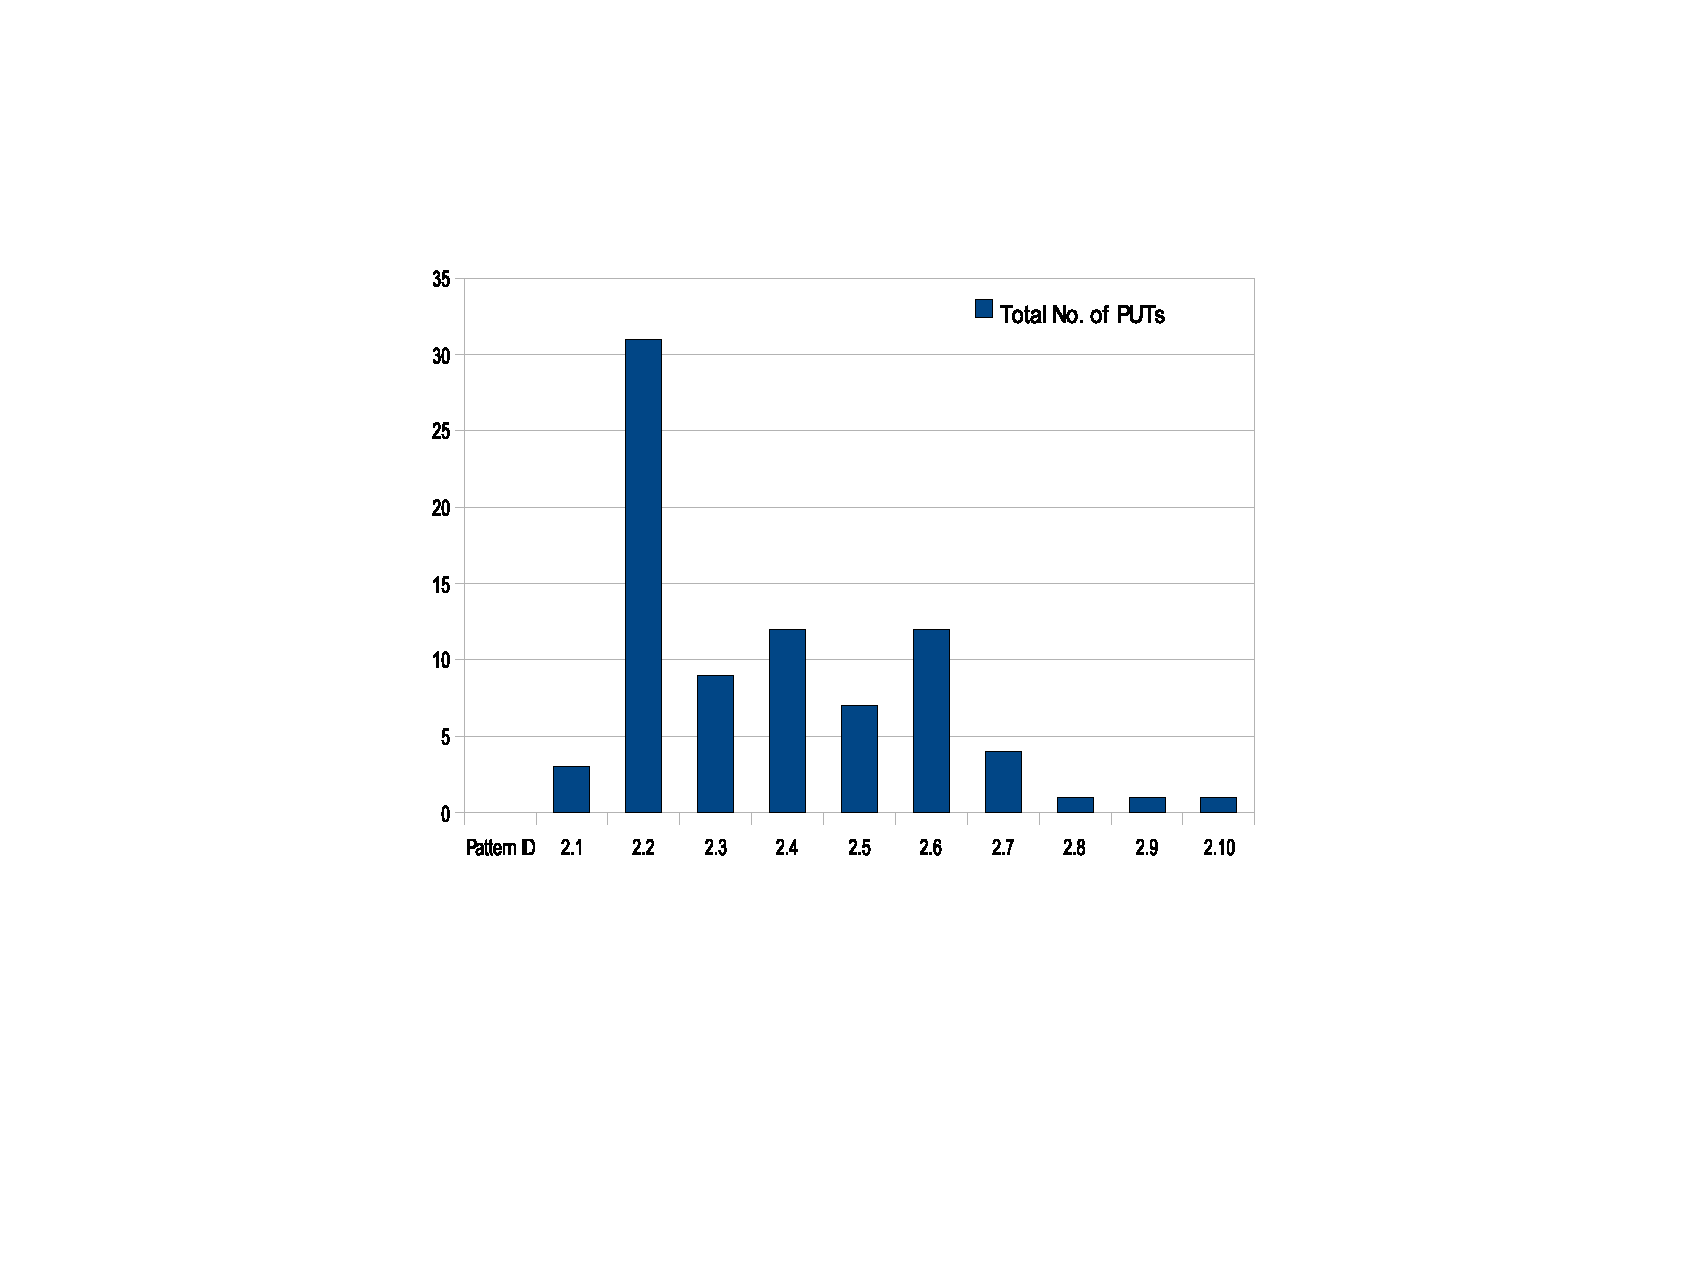
\includegraphics[scale=0.55,clip,trim=180 180 150 100]{figs/patterndistributionSeparated.eps}
\caption{\label{fig:patterndistribution}Distribution of test patterns for 70 PUTs. \textit{The distribution shows that in our testing, only patterns from 2.1 to 2.9 were used.}}
\end{figure}
%---------------------------------------------------------------------------------------
\subsection{New Patterns}
\label{sec:newpatterns}

We next describe two new patterns that can be supported, and that we found useful during our test generalization for the NUnit framework. 
%-------------------------------------------------------------------------------------------
\subsubsection{Random Selection of Cached Values}
\emph{Purpose}: To reuse generated values by maintaining a pool and randomly picking from those values.
\newline
\emph{Motivation}: We next show the motivation for such a pattern with an illustrative example. In the test generalization phase, we needed to generalize an existing unit test 
that requires to verify whether adding a \CodeIn{RegisterKey} to an \CodeIn{NUnitRegistry} and 
then clearing the \CodeIn{NUnitRegistry} work as expected. The \CodeIn{NUnitRegistry} class holds \CodeIn{RegisterKeys} as a tree structure with a main key and an unrestricted number of subkeys in a tree-structured form. Manually adding values and creating a tree structure to check both horizontal and vertical cases at the same time was possible in the existing conventional unit test. However, when the test was parameterized, we were able to write a PUT to add all \CodeIn{RegisterKeys} either to one main key or add each \CodeIn{RegisterKey} to the last added key. Due to such restriction, the unit tests generated by this PUT
resulted in a reduced block coverage when compared to the conventional unit test, although there are a number of tests generated for the PUT. The rationale is that the tests generated for the PUT are expected to generate
a tree structure of keys to achieve high code coverage. As the existing test 
patterns do not meet our current requirement, we proposed a new pattern
where we maintain a pool of existing \CodeIn{RegisterKeys} and randomly
select a key from this pool to add the newly created key as a subkey.
Our new pattern can help construct several forms of tree structures automatically.
Although we explain our motivation using the \CodeIn{RegisterKeys} test
example, our pattern is general and can be applied to tests that require
to reuse previously generated values.
\newline
\emph{Proposed Pattern}: When the input is of the type collection or an array and the values need to be reused by the code under test, 
the values generated by Pex can be added to a pool using our proposed method 
\CodeIn{PexStore.Pool(<name>,<value>)}. \CodeIn{PexStore.Pool()} method is expected to cache values (represented by \CodeIn{value}) for a particular variable (represented by \CodeIn{<name>}). Later, a value can be picked randomly from these cached values using another proposed method \CodeIn{PexStore.Pick(<name>)}. \CodeIn{PexStore.Pick()} method is expected to pick a value randomly from the cached store of the variable \CodeIn{<name>}. Figure~\ref{fig:treepattern} shows an application of our proposed pattern.

\begin{figure}[t]
\begin{CodeOut}
\begin{alltt}
00:[PexMethod()]
01:public void TestClearRoutinesPUT([PAUT]String[] key) \{
02:\hspace*{0.1in}PexAssume.IsTrue(key.Length > 1);
03:\hspace*{0.1in}for (int j = 0; j < key.Length; j++) \{
04:\hspace*{0.3in}PexAssume.IsNotNull(key[j]);
05:\hspace*{0.1in}\}
06:\hspace*{0.1in}NUnitRegistry.TestMode = true;
07:\hspace*{0.1in}using (RegistryKey mainKey = 
08:\hspace*{0.3in}NUnitRegistry.CurrentUser) \{
09:\hspace*{0.3in}//enabling appending values to a list
10:\hspace*{0.3in}\textbf{PexStore.Pool("keys",mainKey)}; 
11:\hspace*{0.3in}for (int j = 0; j < key.Length; j++) \{
12:\hspace*{0.5in}RegisterKey parentKey = 
13:\hspace*{0.7in}\textbf{PexStore.Pick("keys")} as RegisterKey;
14:\hspace*{0.5in}RegistryKey subKey = 
15:\hspace*{0.7in}mainKey.CreateSubKey(key[k - 1]);
16:\hspace*{0.5in}\textbf{PexStore.Pool("keys",subKey)};
17:\hspace*{0.3in}\}
18:\hspace*{0.3in}NUnitRegistry.ClearTestKeys();
19:\hspace*{0.3in}PexAssert.IsTrue(mainKey.SubKeyCount == 0);
20:\hspace*{0.1in}\}
21:\}
\end{alltt}
\end{CodeOut}
\Caption{A new test pattern that helps reuse previously generated values using a cache. \textit{The \CodeIn{PexStore.Pool()} method can be used to append the value \CodeIn{mainKey} to the cache of variable~\CodeIn{keys} and \CodeIn{PexStore.Pick()} method can be used to pick a random value from the cache of the variable \CodeIn{keys}}.}\label{fig:treepattern}
\end{figure}
%------------------------------------------------------------------------------------------------------------
\subsubsection{Unique-value generation}
\emph{Purpose}: To generate unique values when a parameter is a collection of values instead of a single value.
\newline
\emph{Motivation}: In our test generalization phase, for four PUTs, we were unable to achieve the same test effectiveness (i.e., block coverage) by the generated conventional unit tests as that of the existing unit tests. We found the reason to be a required object state: the required object state for the four PUTs to achieve high block coverage can be created only when a unique set of elements is available. For such PUTs, we had to write additional
code to ensure that Pex generates only unique values. For example, in the following PUT, we include a \CodeIn{for} loop with a \CodeIn{PexAssume} (as shown below) on each element of the collection to make sure that
Pex generates a set of unique values. 

\begin{CodeOut}
\begin{alltt}
//PAUT: PexAssumeUnderTest
01:public void SubstorageSettingsPUT1(
\hspace*{0.3in}[PAUT]String subName, [PAUT]String[] name)
02:\{
03:\hspace*{0.3in}PexAssume.IsNotNull(value); 
04:\hspace*{0.3in}PexAssume.IsTrue(name.Length == value.Length);
\hspace*{0.4in}/*assist Pex to generate unique values by 
							 **iterating over each array element and adding
							 **the assumption it is not equal to any other 
							 **array element*/
05:\hspace*{0.3in}for (int i = 0; i < name.Length; i++) \{
06:\hspace*{0.5in}for (int j = 0; j < name.Length; j++) \{
07:\hspace*{0.6in}PexAssume.IsFalse(name[i].Equals(name[j]));
08:\hspace*{0.5in}\}
09:\hspace*{0.3in}\}
10:\hspace*{0.1in}......
11:\}
\end{alltt}
\end{CodeOut}

\emph{Proposed Pattern}: When the input is of the type collection or an array, 
we propose a new pattern using a custom attribute called \CodeIn{PexGenerateUnique} that can inform
Pex to generate unique values. For example, applying the proposed pattern to the preceding example can
result in the following easy-to-write code. We also assume that 
\CodeIn{PexGenerateUnique} subsumes the properties of \CodeIn{PexAssumeUnderTest}.

\begin{CodeOut}
\begin{alltt}
//PAUT: PexAssumeUnderTest
01: public void SubstorageSettingsPUT1([PAUT]String 
\hspace*{0.3in}subName, [\textbf{PexGenerateUnique}]String[] name)
02:\{
03:\hspace*{0.3in}PexAssume.IsNotNull(value); 
04:\hspace*{0.3in}PexAssume.IsTrue(name.Length == value.Length);
05:\hspace*{0.1in}.....
06:\}
\end{alltt}
\end{CodeOut}

For the four PUTs that required generation of a set of unique values, we could apply the proposed pattern as shown in the preceding code example and achieve the test effectiveness.

%----------------------------------------------------------------------------------------------
\section{Patterns and Supporting Techniques}
\label{sec:helper}

We next detail on the PUT patterns and supporting techniques that can be used in writing PUTs. In our study, we primarily use patterns to help generalize test oracles. In addition, we use the supporting techniques of factory methods and mock object to deal with the issues of desirable object states and interactions of the code under test with the environment, respectively. We next describe these techniques in detail.

%-------------------------------------------------------------------------
\subsection{PUT Patterns}
\label{sec:patterns}

A major challenge of writing PUTs is writing a generalized test oracle. When writing CUTs, it is not challenging to write test oracles since for a particular CUT, expected output values can be easily determined for the given input test data based on the method under test. In contrast, when testing with PUTs, determining the expected output values is not trivial; a PUT should be designed to assert output values based on a number of input values generated by Pex for that PUT. To address this issue, we propose $15$ PUT patterns~\cite{halleux08:putpatterns} that help developers to deal with this issue of generalizing test oracles. Table~\ref{tab:patterns} shows $13$ of the proposed $15$ PUT patterns\footnote{The other two PUT patterns are related to regression testing, which is not within the scope of our paper.}.

\setlength{\tabcolsep}{2pt}
\begin{table}[t]
\begin{center}
\begin {tabular} {|r|l|}
\hline
									\#			&	Pattern Name									\\				%&	Pex Supported Attributes or Methods\\
\hline
\hline
									1				&	Arrange, Act, Assert (AAA)					\\				%&	\\
\hline
									2				&	Assume, Arrange, Act, Assert (AAAA) 	\\			%&	\\
\hline
									3				&	Constructor Test							\\				%&	\\
\hline
									4				&	Roundtrip											\\				%&	\\
\hline
									5				&	Sanitized Roundtrip						\\				%&	\\
\hline
									6				&	State Relation								\\				%&	\\
\hline
									7				&	Same Observable Behavior			\\				%&	\\
\hline
									8				&	Commutative Diagram						\\					%&	\\
\hline
									9				&	Cases													\\					%&	PexAssert.Case() 			\\ 
\hline
									10			&	Allowed Exception							\\					%&	[PexAllowedException]	\\
\hline
									11			&	Reachability									\\					%&	[PexExpectedGoals]		\\
\hline
									12			&	Parameterized Stub						\\					%&	[PexAssumeUnderTest]	\\
\hline	
									13			&	Manual Output Review					\\					%&	PexObserve.Value			\\
\hline
%									14			&	Regression Tests							\\					%&	PexStore.ValueForValidation()\\
%\hline
%									15			&	Differential Regression Test Suite	\\%&	\\
%\hline
\end{tabular}
\caption {\label{tab:patterns} PUT Patterns}  \vspace*{-3ex}
\end{center}
\end{table}

The proposed PUT patterns serve two purposes: (1) they assist in designing a PUT based on the developers' test objective, and (2) they assist in determining test oracles that can deal with the generality of the PUT. Patterns 1, 2, 9, 10, and 11 (shown in Table~\ref{tab:patterns}) primarily assist developers in designing PUT based on the test objective. For example, developers can use Pattern 2 (AAAA) when the method under test needs to be tested for a particular range of input values (the PUT includes assumptions), and the behavior of the method under test can be asserted using assertion statements (the PUT includes assertions). Similarly, developers can use Pattern 10 (Allowed Exception) when a method under test may throw a particular exception, and such an exception being raised does not indicate that the unit test fails. 
The remaining patterns listed in the table assist developers in writing test oracles. For example, developers can use Pattern 6 (State Relation) when a method under test causes an internal change to the object state, which in turn can be observed through other methods. 

\begin{figure}
\begin{CodeOut}        
\begin{alltt}
01: public void Clear() \{
03: \hspace{0.07in}root = null;
04: \hspace{0.07in}Count = 0;
05: \}
\end{alltt}        
\end{CodeOut}\vspace*{-4ex}
\caption{\CodeIn{Clear} method of \CodeIn{AvlTree} class of DSA.}
\label{fig:pattern}%

\begin{CodeOut}        
\begin{alltt}
01: public void ClearCUT() \{
03: \hspace{0.07in}AvlTree<int> actual = new AvlTree<int>\{1,3,5,6,9,7\};
04: \hspace{0.07in}Assert.AreEqual(6, actual.Count);
05: \hspace{0.07in}actual.Clear();
06: \hspace{0.07in}Assert.AreEqual(0, actual.Count);            
07: \}
\end{alltt}
\end{CodeOut}\vspace*{-4ex}
\caption{Existing CUT to test the \CodeIn{Clear} method.}%
\label{fig:patternCUT}%
\end{figure}

We next illustrate the use of PUT patterns in designing a PUT and in determining a test oracle. Figure~\ref{fig:pattern} shows the \CodeIn{Clear} method from \CodeIn{AvlTree} of the DSA~\cite{dsa} library. The \CodeIn{Clear} method clears the contents of the \CodeIn{AvlTree} object. Figure~\ref{fig:patternCUT} shows the existing CUT to test the \CodeIn{Clear} method. The objective of the CUT is to create an \CodeIn{AvlTree} object with the given list of items, invoke the \CodeIn{Clear} method, and assert if the elements are removed. To transform this CUT to a PUT, developers promote the input list to the constructor of \CodeIn{AvlTree} as a parameter to the PUT. Based on the test objective, developers identify two patterns to write the PUT: (1) AAAA, there should be an assumption on the parameter since the parameter should be non-null, and the result of the \CodeIn{Clear} method should be asserted, and (2) State Relation, since the behavior of the \CodeIn{Clear} method can be observed using the \CodeIn{Count} field, i.e., observe the change in the object state. Using the identified patterns, developers can write a PUT shown in Figure~\ref{fig:patternPUT}. 

\begin{figure}
\begin{CodeOut}        
\begin{alltt}
01: public void ClearPUT([PAUT]List<int> values) \{
03: \hspace{0.07in}AvlTree<int> actual = new AvlTree<int>(values);
04: \hspace{0.07in}PexAssert.AreEqual(values.Count, actual.Count);
05: \hspace{0.07in}actual.Clear();
06: \hspace{0.07in}PexAssert.AreEqual(0, actual.Count);
07: \}
\end{alltt}
\end{CodeOut}\vspace*{-4ex}
\caption{PUT transformed from CUT in Figure~\ref{fig:patternCUT}, using the AAAA and State Relation patterns.}%
\label{fig:patternPUT}%
\end{figure}

%-------------------------------------------------------------------------
\subsection{Factory Methods}
\label{sec:factory}

Pex often faces challenges in handling PUT parameters of complex non-primitive types, because these parameters require method-call sequences (that create and mutate objects of non-primitive types) to generate desirable object states. These desirable object states are the states that help explore new paths or branches in the code under test. For example, a desirable object state to cover the \CodeIn{true} branch of Statement 8 in Figure~\ref{fig:cut} is that the \CodeIn{storage} object should already include a value for the setting name \CodeIn{sn}. Althrough Pex includes static analysis to generate sequences of public method calls that aim at initializing all fields of an object, such a fixed sequence in not appropriate in all scenarios.
%Although Pex includes a demand-driven strategy for generating method-call sequences, Pex's strategy can generate method-call sequences effectively in certain limited scenarios where the constructors either accept primitive parameters or explicitly state the actual type of the parameter.

To assist Pex in generating effective method-call sequences that can help achieve desirable object states, developers can write method-call sequences inside factory methods, supported by Pex. Such factory methods can have parameters, and then Pex determines a set of relevant argument values for factory methods just as Pex does for PUTs. Figure~\ref{fig:factorymethd} shows an example factory method for the \CodeIn{MemorySettingsStorage} class. The factory method accepts two arrays of setting names (\CodeIn{sn}) and values (\CodeIn{sv}) and adds these entries to the storage. This factory method helps Pex to generate method-call sequences that can create desirable object states. For example, Pex can generate five names and five values as arguments to the factory method for creating a desirable object state with five elements in the storage\footnote{Note that the factory methods provide only an assistance to Pex in achieving the desirable object states, and Pex generates these object states based on the branching conditions in the code under test.}. The same factory method can be reused for all other PUTs using the \CodeIn{MemorySettingsStorage} class as parameter types.

%-------------------------------------------------------------------------
\subsection{Mock Objects} 
\label{sec:mock}

A mock object~\cite{mockobjects} is an implementation for simulating environments such as file systems. Mock objects help test unit behaviors in isolation where the interactions of the unit under test with the real environment are replaced with the mock objects\footnote{Unit tests with such mock objects do not replace integration tests. However, mock objects are the only way to test environment-dependent code in isolation in unit testing.}. Automatic test generation tools such as Pex could require various desirable environment states to generate unit tests that achieve high code coverage. Creating these desirable environment states requires extensive test setup. Since such test setup can generate a lot of garbage in the environment (such as adding extra files in the file system), a significant amount of test cleanup is also required. We next describe how developers can use mock objects with an example from our study. 

\begin{figure}
\begin{CodeOut}
\begin{alltt}
01: public class MockXmlTextWriter \{ 
02:\hspace*{0.1in}public MockXmlTextWriter(string filename,
\hspace*{0.25in} Encoding encoding) \{ 
04:\hspace*{0.3in}this.fileName = filename;
05:\hspace*{0.1in}\}

06:\hspace*{0.1in}public void WriteAttributeString
\hspace*{0.3in}(string attributeName, string value) \{
08:\hspace*{0.3in}xmlString = xmlString + " " + attributeName 
\hspace*{0.7in}+ "=" + "\"" + value + "\"";
09:\hspace*{0.1in}\}

10:\hspace*{0.1in}public void Close() \{
12:\hspace*{0.3in}xmlString = xmlString.Replace("/> />", "/>" + 
   \hspace*{0.5in}System.Environment.NewLine + "</" 
   \hspace*{0.7in}+ startString + ">");
13:\hspace*{0.3in}CreatedProjects.currentProject = xmlString;
14:\hspace*{0.1in}\}
\hspace*{0.3in}............
15: \}
\end{alltt}
\end{CodeOut}  \vspace*{-3ex}
\caption{\label{fig:mockobject} Sample code from the \CodeIn{MockXmlTextWriter} mock object. In the \CodeIn{WriteAttributeString} method, the argument string is appended to a global string \CodeIn{xmlString} and this global string represents the content written to the xml file.}  \vspace*{-3ex}
\end{figure}

In the \CodeIn{NUnitProject} class of the NUnit application, to test the \CodeIn{save} method, the developer can use a mock object to replace the interactions of code under test with the \CodeIn{XmlTextWriter}. The purpose of the \CodeIn{save} method is to write configuration information to an XML file. This XML file is expected to be created when the project is created, i.e., an instance of \CodeIn{NUnitProject} is created. Two existing CUTs \CodeIn{SaveEmptyConfigs} and \CodeIn{SaveNormalProject} test this \CodeIn{save} method. These CUTs add configurations to the XML project files and assert whether the files are saved in the right format and contain the added configuration information. Both the CUTs depend on a default empty project that is created using the test setup method. Therefore, the requirement to test the \CodeIn{save} method is to provide the project configuration file (the XML file) in a \emph{specific location}, i.e., the directory location where the project is saved (when a project is saved, a new directory is created as the project directory and the XML file is created in this directory). 

To generalize these CUTs, the developer can promote the project path (a parameter to the \CodeIn{save} method and a local variable in the CUTs) as a parameter to the PUT. However, generalization of these CUTs is not straightforward. By promoting the project path as the PUT's paramater, every unit test generated by Pex using the PUT requires an XML file in the location (reflected by the generated value for the parameter). The reason is that when the \CodeIn{save} method is invoked, the XML file is accessed using \CodeIn{XmlTextWriter}. Without the XML file, the \CodeIn{save} method throws an exception. Therefore, to avoid the complexity of creating a ``real'' file at a ``real'' location and to prevent the exception thrown by the \CodeIn{save} method, the developer can mock the expected behavior of \CodeIn{XmlTextWriter} with \CodeIn{MockXmlFileWriter}. This mock object simulates the behavior of \CodeIn{XmlTextWriter}, but unlike the real object, it appends the input text to a \CodeIn{string}, still preserving the output of the actual behavior of \CodeIn{XmlTextWriter}, and avoiding the interactions with the file system. Figure~\ref{fig:mockobject} shows a code snippet of the \CodeIn{MockXmlTextWriter} class. By using the mock-object technique, the developer can achieve generalization of both the CUTs to test the \CodeIn{save} method.

%The \CodeIn{xml} file was expected to already exist physically for the test to execute so that the code under test can access the file and add configuration information to the file, and test if the project is correctly saved with the configurations. The existing tests save the projects and assert by reading the \CodeIn{xml} file using a stream reader and check against an expected string (which is constructed based on the configurations that are added). 
%------------------------------------------------------------------------------------------------------

%\subsection{Input-Space Partitioning}
%\label{sec:inputspace}
%
%Input-space partitioning~\cite{paul:offut} helps partition the input space into disjoint blocks,
%where the union of all the blocks should result in the complete input space.  
%We explain how we performed the input-space partitioning in our study to achieve
%a higher coverage of the method \CodeIn{SaveSetting} of the class
%\CodeIn{SettingsGroup}. The \CodeIn{SaveSetting} method accepts an argument of type
%\CodeIn{Object}. The method accepts several types such as \CodeIn{int}, \CodeIn{string},
%\CodeIn{bool}, and \CodeIn{enum}, and a different path of the code is covered for each type. Therefore, in order to achieve high code coverage, a PUT to test this method should be designed to generate conventional unit tests that take different types of the argument. For simplicity, we explain how we dealt with
%integers and strings only. We defined two partitions where the first partition includes
%integers and the second partition includes strings. We wrote separate PUTs for
%covering these partitions. We repeated the same procedure for other input types. Consequently, Pex achieved high coverage as it was able to generate different input types and cover several program paths.
%----------------------------------------------------------------------------
%\subsection{Delegates} 
%\label{sec:delegate}
%
%Delegates are used to encapsulate a method with a specific signature and 
%a return type. These delegates are used to pass methods as arguments instead
%of data, which is commonly used in practice. Such a feature is quite helpful
%when the method to be called is known \emph{only} during runtime. These delegates
%feature is often used in GUI applications for event-handling. In our study, we found that some code portions are not covered as those portions require the delegates
%to be defined. We next show an example delegate class we used in Phase 2 of our study.
%% We expect that Pex can be easily extended to provide support for
%%delegates also. We next explain how Pex can be extended to provide such support
%%with illustrative examples. 
%\begin{figure}
%\begin{CodeOut}
%\begin{alltt}
%00:namespace Application \{
%01:\hspace*{0.1in}public delegate int MyHandler(object sender, 
%02:\hspace*{0.8in}MyEventArgs e);
%03:\hspace*{0.1in}class DelegateClass \{
%04:\hspace*{0.2in}public int DMethod(object sender, MyEventArgs e)\{
%05:\hspace*{0.3in}Console.WriteLine("In Delegate {0}", e.m_id);
%06:\hspace*{0.2in}\}
%07:\hspace*{0.2in}public A(TestCls b)\{
%08:\hspace*{0.3in}MyHandler d1 = new MyHandler(DMethod);
%09:\hspace*{0.3in}b.Event += d1;
%10:\hspace*{0.2in}\} 
%11:\hspace*{0.1in}\}
%12:\hspace*{0.1in}class TestCls \{
%13:\hspace*{0.2in}public event MyHandler Event;        
%14:\hspace*{0.2in}public void MUT(MyEventArgs e)\{
%15:\hspace*{0.3in}if (Event != null) \{
%16:\hspace*{0.4in}Event(this, e); \}
%17:\hspace*{0.3in}\}
%18:\hspace*{0.2in}\} 
%19:\hspace*{0.1in}\}
%20:\}
%\end{alltt}
%\end{CodeOut}
%\Caption{\label{fig:delegateex} A code example with a delegate handler.}
%\end{figure}
%
%Figure~\ref{fig:delegateex} shows two classes \CodeIn{DelegateClass}
%and \CodeIn{TestCls}. \CodeIn{TestCls} defines a method under test
%with the name \CodeIn{MUT}. When the method \CodeIn{MUT} is executed 
%without defining any delegate handler, Pex cannot cover Statement 16. 
%We manually created a delegate handler 
%with the name \CodeIn{DelegateClass} and added the handler using
%the operator \CodeIn{+=} as shown in Statement 9. These delegate handlers
%are different from normal method calls as there can be multiple delegate handlers
%that can be registered for one event. 
%Pex can be extended 
%to provide additional feature to automatically take care of
%delegate handlers. Pex can generate mock methods based on the signature
%of delegate (shown in Statement 1). For example, Pex can generate a
%mock method with argument types \CodeIn{object} and \CodeIn{MyEventArgs}
%with the following code inside the method.

%\begin{CodeOut}
%\begin{alltt}
%\hspace*{0.1in}var chooser = PexChoose.FromCall(this);
%\hspace*{0.1in}return chooser.ChooseResult<int>();
%\end{alltt}
%\end{CodeOut}

%The preceding method can replace the manually written delegate handler
%shown in Statements 3 to 11 in Figure~\ref{fig:delegateex}.
%The reason for using \CodeIn{PexChoose} in the automatically generated
%mock methods is that Pex can later infer the return value of the mocked
%delegate handler based on the further branch conditions in the source code.
%Sometimes, there can be more than one delegate handler associated with 
%each event such as the method call \CodeIn{Event} in Statement 16. Pex can
%simulate such behavior by defining multiple mock methods for
%each \CodeIn{Event}. One issue that can arise is that when there are multiple
%delegate methods for each \CodeIn{Event}, there can be multiple return values.
%In this scenario, C\# documentation suggests to use the return value
%that is returned from the last delegate.
%----------------------------------------------------------------------------------------------
\section{Benefits of PUTs}
\label{sec:newbenefits}
We next present the benefits of retrofitting conventional unit tests for PUTs. 
In test generalization, we transformed 57 conventional unit tests of 10 test classes resulting in 49 PUTs.  In order to achieve higher block coverage, we wrote 21 new PUTs for 6 of the 10 classes under study. Table~\ref{tab:oldbenefits} shows the results of writing PUTs. Column ``Test Class'' shows the names of the test class and Column ``Test Methods'' shows the statistics of existing 
conventional test methods, the test methods that are amenable to 
test generalization, the percentage of amenable conventional unit tests, the number of transformed PUTs, and the number of new PUTs that were written. The five sub-columns 
represented by ``Conventional'', ``\#Amenable'', ``\%'', ``\#PUT'', and ``\#New PUT'' give cumulative figures for all test methods in the corresponding class. ``\#PUT'' shows the number of PUTs written in Phase 1 and ``\#New PUT'' shows the number of new PUTs written in Phase 2 to achieve higher coverage. Section~\ref{sec:notamenable} provides details of the test methods that are not amenable to test generalization with illustrative examples. 
Column ``\% Coverage'' shows the block coverage reported by Pex on executing
tests. These two sub-columns show the average of all the test methods in each class. Column ``Avg. New Blocks'' 
shows the average number of new blocks covered by PUTs. As PUTs can verify more general behavior,
we found that PUTs achieve a high block coverage and cover new blocks
that are not covered by conventional unit tests. Column ``\#Defects'' shows the number of defects that were detected by the PUTs 
and were not detected by the existing conventional unit tests. 
This column again shows a cumulative value of all the test methods in a test class.
%---------------------NEW TABLE SHOWING THE BENEFITS OF TEST GENERALIZATION-----------------------
\setlength{\tabcolsep}{2pt}
\begin{table*}[t]
\begin{center}
\centering \caption {\label{tab:oldbenefits} Benefits of Retrofitting PUTs in Unit Testing} \vspace*{0.1in}
\begin {tabular} {|l|r|r|r|r|r|r|r|r|r|r|}
\hline
Test Class						&\multicolumn{5}{|c|}{Test Methods}				& \multicolumn{3}{|c|}{\% Coverage}						&Avg. New	&\#Defects\\
								 			&\multicolumn{5}{|c|}{}										&	\multicolumn{3}{|c|}{}											&Blocks		&\\
\cline{2-9}
											&\#Conventional	&\#Amenable		&\%					&\#PUT		&\#New PUT		&Conventional	&PUT		&With			&		&\\
											&								&							&						&					&							&							&				&New PUT	&		&\\
\hline
NUnitProjectSave.cs		&3							&1						&33.33			&1				&2						&35.71				&40.98	&57.91		&10		&0\\
\hline
NUnitRegistryTests.cs	&5							&5						&100.00			&4				&							&58.97				&72.80	&100.00		&0		&1\\
\hline
TestAgentTests.cs			&2							&2						&100.00			&2				&1						&100.00				&100.00	&NA				&0		&0\\
\hline
RegistrySettings-			&								&							&						&					&							&							&				&					&			&	\\
StorageTests.cs				&6							&5						&83.33			&6				&4						&45.34				&90.60	&100.00		&0		&1\\
\hline
MemorySettings-				&								&							&						&					&							&							&				&					&			&	\\
StorageTests.cs				&6							&4						&66.67			&4				&							&100.00				&100.00	&NA				&2		&0\\
\hline
PathUtilTests.cs			&7							&3						&42.86			&6				&							&85.00				&85.00	&NA				&0		&3\\
\hline
RecentFilesTests.cs		&22							&21						&95.45			&5				&6						&59.94				&76.08	&84.17		&14		&0\\
\hline	
ServerUtilityTests.cs	&2							&2						&100.00			&3				&1						&90.32				&90.32	&95.16		&0		&2\\
\hline
SettingsGroupTests.cs	&5							&5						&100.00			&6				&7						&66.94				&90.95	&94.13		&2		&0\\
\hline
ProcessRunnerTests.cs	&0							&NA						&NA					&NA				&NA						&NA						&NA				&NA			&NA		&NA\\
\hline
\end{tabular}
\end{center}
\end{table*}
%-------------------------------------------------------------------

The benefits discussed here primarily reflect the results of the test generalization phase as we compare the benefits of PUTs over the existing conventional unit tests. Section~\ref{sec:limitations} discusses the amount of effort we took in writing the new PUTs in comparison to generalizing the existing conventional unit tests. We found three major benefits of retrofitting conventional unit tests for PUTs: higher code coverage, detection of new defects, and reduced test code. We observed that generalization
increases code coverage and detected new defects that were not
detected by the existing conventional unit tests. 
We also identified that
a single PUT often helps to replace multiple conventional unit tests,
thereby reducing the amount of test code (as shown by Column ``\#Convention'' and Column ``\#PUT'' in Table~\ref{tab:oldbenefits}). Sections~\ref{sec:coverage}, \ref{sec:defects}, and \ref{sec:testcode} explain these details.
%-------------------------------------------------------------------
\subsection{Coverage}
\label{sec:coverage}

As generalized tests often help cover more scenarios, we found that
test generalization helped to have an effective increase in the block coverage as shown in Table~\ref{tab:oldbenefits}.
For example, test generalization of the \CodeIn{RegistrySettingsStorage}
class shows an increase in the coverage of 45.24\%.
In addition, the tests generated for the PUTs in the test generalization achieved coverage
of new blocks that are not covered by the existing conventional 
unit tests. In order to achieve more code coverage, we wrote 21 new PUTs for 6 classes and obtained an average increase of $35$\% code coverage (considering only those classes for which we wrote new PUTs).
%For example, the generalization of conventional
%unit tests in the \CodeIn{RecentFilesTests.cs} covered $14$
%additional blocks (on average for all PUTs). In one scenario of \CodeIn{RecentFilesTest.cs}, there is a decrease in the \% of coverage when the conventional unit tests were transformed to PUTs; however, there is a significant increase in the number of blocks covered by the PUTs. The decrease in the coverage is due to the increase in the number of blocks covered by the PUT when compared to the corresponding conventional unit-test. The difference is primarily due to the
%Pex strategy of reporting block coverage as Pex cannot detect the total number of blocks correctly
%when some methods are not analyzed. For example, the numbers of blocks covered by two PUTs in the \CodeIn{RecentFilesTest.cs} were 56 and 58, while the conventional unit tests accounted for 23 and 25, respectively. The ratio of blocks covered to the total number of blocks accounted by PUTs are 41/56 (73.21\%) and 41/58 (70.69\%). Similarly, for conventional unit tests the ratio was 18/23 (78.26\%) and 18/25 (72.00\%). Therefore, despite an increase in the total number of blocks covered, there is a decrease in the \% of code coverage. 
%Benefits of adding new PUTs was not only an increase in the code coverage, but also we were able to write new PUTs for three conventional unit tests, which were not amenable to test generalization.
%-------------------------------------------------------------------
\subsection{Defects}
\label{sec:defects}

After test generalization we found 7 new defects that were not detected by
the existing conventional unit tests. We next explain a defect detected 
by our test generalization. The \CodeIn{NUnitRegistry} 
class stores the \CodeIn{RegistryKeys} in a tree-structured hierarchy. 
For building the key hierarchy, a default key is taken as a main 
key and the given keys are added as sub-keys to the main key or to the other sub-keys. During testing, adding a key hierarchy and on checking for the count or on clearing the keys, we found abnormal behavior for two tests. The PUT was written to take three test inputs. For one of the tests generated by Pex, the test inputs were \CodeIn{t}, \CodeIn{t}, and \CodeIn{t}, and the other test case took the test inputs as \CodeIn{$\backslash$0}, \CodeIn{$\backslash$0}, and \CodeIn{$\backslash$0}. For the first test case, when the three inputs were added to a main key (two as sub-keys and the other as a sub-key to one of the added subkeys), the count check for the keys passed, i.e., \CodeIn{PexAssert(2, mainKey.SubKeyCount)} passed. The same assertion failed for the second case (with test inputs ``$\backslash$0'') with an assertion failure message, ``expected 2, got 1''. This defect shows that the failure was possibly due to missing check on invalid characters. 
%-------------------------------------------------------------------
\subsection{Test Code}
\label{sec:testcode}

Test generalization also helped reduce the 
test code as shown in Column ``\#PUT'' of Table~\ref{tab:oldbenefits}. Often, test
generalization either helps reduce the amount of code in a single test method or
helps combine multiple test methods into a single PUT. Figure~\ref{fig:caseput}
shows an example PUT of the pattern type \emph{Cases} that combined five conventional unit tests. Each conventional
unit test verifies one case in the corresponding PUT. In addition, the PUT achieved higher coverage compared
to the five conventional unit tests as the \CodeIn{MaxValue} is now accepted
as an argument and the concrete values are generated from the argument
based on captured constraints.

\begin{figure}[t]
\begin{CodeOut}
\begin{alltt}
[PexMethod]
public void CountOverOrAtMaxPUT1(int MaxValue) \{
\hspace*{0.1in}recentFiles.MaxFiles = MaxValue;
\hspace*{0.1in}PexAssert
\hspace*{0.2in}.Case(MaxValue < MIN)
\hspace*{0.3in}.Implies(() => MIN == recentFiles.MaxFiles)
\hspace*{0.2in}.Case(MaxValue == MIN)
\hspace*{0.3in}.Implies(() => MaxValue == recentFiles.MaxFiles)
\hspace*{0.2in}.Case(MaxValue > MIN && MaxValue < MAX)
\hspace*{0.3in}.Implies(() => MaxValue == recentFiles.MaxFiles)
\hspace*{0.2in}.Case(MaxValue == MAX)
\hspace*{0.3in}.Implies(() => MaxValue == recentFiles.MaxFiles)
\hspace*{0.2in}.Case(MaxValue > MAX)
\hspace*{0.3in}.Implies(() => MAX == recentFiles.MaxFiles);            
\} 
\end{alltt}
\end{CodeOut}
\Caption{\label{fig:caseput} Single PUT constructed from five conventional tests.}
\end{figure}

%----------------------------------------------------------------------------------------------
\section{Conventional Unit Tests Not Am- enable to Test Generalization} 
\label{sec:notamenable}

In our study, we found that $12.75$\% of conventional unit tests are not amenable to test generalization. There are two common cases under which we found that conventional unit tests are not amenable to test generalization. 

\textbf{Default checks.} We found that there are multiple conventional unit
tests that verify default values, which are often static values. We suspect
that the purpose of these tests could be to make sure that the developers do not
change the static values accidentally. We suspect that these tests are
not amenable for test generalization as values verified by these tests
are constants.

\textbf{Missing test oracles.} We found that test generalization
may cause the loss of test oracles in some cases. These cases can often occur when generalizing conventional unit tests that belong to the PUT patterns \emph{Roundtrip} and \emph{Commutative diagram}.
We explain this issue using the illustrative example shown below.

\begin{CodeOut}
\begin{alltt}
public void Canonicalize() \{
\hspace*{0.1in}PexAssert.AreEqual(@"C:/folder1/file.tmp",
\hspace*{0.3in}PathUtils.Canonicalize(@"C:/folder1/./folder2/
\hspace*{0.3in}../file.tmp")); 
\}
\end{alltt}
\end{CodeOut}
 
The \CodeIn{Canonicalize} method in \CodeIn{PathUtils} accepts
a \CodeIn{string} parameter and uses a complex procedure to transform the input \CodeIn{string} into a standard form. It is easy to identify the expected output for concrete strings
such as ``\CodeIn{C:/folder1/.../folder2/.. ./file.tmp}''. However, when the
conventional unit test is generalized with a parameter for the input string, it is challenging to 
identify the expected output. Developers need to implement a logic to assert the behavior of the method under test. The amount of effort required in such cases could be higher than the effort required to write the implementation of the actual method under test and therefore such conventional unit tests are not amenable to test generalization.

%----------------------------------------------------------------------------------------------
\section{Discussion} 
\label{sec:limitations}

In our results related to test-code maintenance, there is a scenario where the number of PUTs is more than the number of CUTs. The reason is that it is sometimes difficult to generalize test oracles in a few cases. For example, consider the following CUT:\vspace*{-1.5ex}

\begin{CodeOut}
\begin{alltt}
public void Canonicalize() \{
\hspace*{0.1in}PexAssert.AreEqual(@"C:/folder1/file.tmp",
\hspace*{0.3in}PathUtils.Canonicalize(@"C:/folder1/./folder2/
\hspace*{0.3in}../file.tmp")); 
\}
\end{alltt}
\end{CodeOut} \vspace*{-1.5ex}

\noindent The \CodeIn{Canonicalize} method in \CodeIn{PathUtils} accepts a \CodeIn{string} parameter and uses a complex procedure to transform the input into a standard form. It is easy to identify the expected output for concrete strings such as \CodeIn{C:/folder1/.../folder2/.../file.tmp}. However, when the CUT is generalized with a parameter for the input string, it is challenging to identify the expected output. Although a developer can use our commutative diagram pattern and provide an alternative implementation for the \CodeIn{Canonicalize} method, the amount of required effort could be higher than the effort required to write the implementation of the actual method under test. To address this issue in our empirical study, we split the CUT into multiple PUTs during test generalization. For those PUTs with difficulties in generalizing test oracles, we do not generalize the test assertions, and instead replace assertions with statements that print outputs suitable for manual review, i.e., use the \emph{manual output review} pattern in our proposed patterns. These PUTs can still help in detecting defects related to exceptions.

In our empirical study, for a PUT generalized from the CUT \CodeIn{GraphWithSelfEdges} (in the \CodeIn{Concepts} namespace of QuickGraph), we identify that the PUT achieved branch coverage of 70\%, which is less than the coverage achieved by the existing CUT. The reason is that the transformed PUT executes a huge amount of code and Pex reached the upper-bound of the number of explored branches (by default, pre-configured to avoid long running of Pex). Although we tried to set higher upper-bound values, Pex was still not able to generate unit tests that achieve higher coverage than the existing CUT. To address this issue, we performed a partial generalization by not promoting the loop bound as a parameter for the PUT. Due to our partial generalization, the transformed PUT achieved a branch coverage of 83\%, which is 11\% higher than the existing CUT.

For NUnit, the LOC of PUTs is more than the LOC of CUTs. The reason is that to transform $2$ CUTs to PUTs, the respective test objectives required \textit{specialized} test data, such as that a tree structure of keys was required to test the \CodeIn{ClearTestKey} method of the \CodeIn{NUnitRegistry} class. In order to create such specialized test data, we created the required test setup that increased the LOC of PUTs for NUnit.

We conducted our empirical study as third-party testers since we do not have the knowledge of the subject applications. We expect that our test-generalization results can be much better if the test generalization is performed by the developers of these subject applications. The reason is that developers can incorporate their domain knowledge during test generalization to write more effective PUTs.

%One of the major limitations of PUTs is that PUTs requires more effort from developers than writing conventional unit tests requires. Although PUTs reduce the complexity of writing multiple conventional unit tests with various concrete test inputs, developers need additional expertise in writing such PUTs as PUTs are more generic compared to conventional unit tests. For example, writing PUTs requires developers to prescribe a test oracle that can deal with the generality of test inputs. We show that to reduce the complexity of writing PUTs, we adopted a methodology of writing PUTs in two phases. In Phase 1, we generalized the existing conventional unit tests to PUTs using suggested test patterns. In Phase 2, we used supporting techniques to write more PUTs to assist Pex in generating high-covering tests. 

%In our study, we observed that we took longer time to write PUTs in Phase 2 compared to the time we took in Phase 1. In Phase 1, we transformed the existing conventional unit tests to PUTs and the existing unit tests assist in writing PUTs as shown in Section~\ref{sec:example} with an example. In Phase 2, we discovered the un-covered code portions and wrote more PUTs to assist Pex to generate tests to cover the un-covered code portions. Based on our experience, we believe that to enjoy the test effectiveness achieved by writing PUTs and to reduce the cost involved in writing PUTs, a practical solution could be retrofitting PUTs by transforming these conventional unit tests to PUTs. We expect that writing a single conventional unit test to test a method under test and then transforming it to a PUT can help developers in writing the PUTs. Such a single conventional unit test can act as an \textit{example} unit test representing the intention of ``what'' needs to be tested. We expect that this methodology can both ease the process of writing PUT and still achieve high test effectiveness in unit testing. 

%As shown in our study, although the usage of the suggested test patterns and the supporting techniques can reduce effort of developers in writing PUTs and allow the test generation tool to generate high-covering tests, the complexity lies in being able to use them. In general, developers might consider it a tougher job to learn the supporting techniques and use them to write PUTs than writing multiple possible conventional unit tests. Nevertheless, our study shows that PUTs are more effective than conventional unit tests in detecting defects and also in achieving high code coverage. Therefore, we believe that the choice of writing PUTs is a trade-off between cost and benefit.
%----------------------------------------------------------------------------------------------
\section{Related Work}
\label{sec:related} In this section, we introduce related work and
discuss our contributions.

\textbf{Language migration.} It is a research topic with a long
history to migrate projects of one language into other
languages~\cite{samet1981experience}. To reduce the human effort of
language migration, researchers propose various approaches to
automate the
process~\cite{van1999identifying,waters1988program,mossienko2003automated,yasumatsu1995spice,hainaut2008migration}.
Most of these approaches focus the syntax differences among
languages. For example, Deursen \emph{et
al.}~\cite{van1999identifying} propose an approach to identify
objects in legacy code, and the results are useful to deal with the
difference  between object-oriented languages and procedural
languages. As shown by El-Ramly \emph{et
al.}~\cite{el2006experiment}'s experience report, existing
approaches and tools support only a subset of APIs, and consequently
it becomes an important to automate API transformation. Our approach
mines API mapping among languages to aid language migration,
complementing the preceding approaches.

\textbf{Library migration.} With the evaluation of libraries, some
APIs may become incompatible. To deal with the problem, some
approaches have been proposed. In particular, Henkel and
Diwan~\cite{henkel2005catchup} propose an approach that captures and
replay API refracturing actions to keep client code updated. Xing
and Stroulia~\cite{xing2007api} propose an approach that recognizes
the changes of APIs by comparing the differences of two versions of
libraries. Balaban \emph{et al.}~\cite{balaban2005refactoring}
propose an approach to help translate client code when mapping
relations of libraries are available. Different from these
approaches, our approach focuses on mapping relations of APIs among
different languages. In addition, as our approach uses ATGs to mine
mapping relations of APIs, our approach helps mine mapping relations
for those API methods whose input orders is changed or whose
functionalities are split into several methods if our approach is
applied in library migration.

%----------------------------------------------------------------------------------------------
\section{Threats to validity}
\label{sec:tov}
\vspace*{2ex}

The threats to external validity primarily include the degree to which the subject programs, faults, and conventional unit tests are representative of true practice. 
The number of classes used in our empirical study is relatively small, although the defects detected during our study are real defects. These threats could be reduced by conducting more studies with wider types of subjects in our future work. The threats to internal validity are due to manual process involved in writing PUTs. Our study results can be biased based on our experience and knowledge of the subject programs. These threats can be reduced by conducting more case studies with more subject programs and other human subjects. The results in our study can also vary based on other factors such as the effectiveness of our written PUTs and test generation capability of Pex. One threat to construct validity is that our study uses the block coverage reports generated by Pex to reflect the quality of tests.
%----------------------------------------------------------------------------------------------
\section{Conclusion}
\label{sec:conclusion}

Mapping relations of APIs are quite useful for the translation
of projects from one language to another language, and
it is difficult to mine these mapping relations due to various
challenges. In this paper, we propose a novel approach that mines mapping
relations of APIs from existing projects with multiple versions in
different languages. We conducted two evaluations to show the effectiveness
of our approach. The results show that our approach mines many API mapping
relations between Java and C\#, and these relations improve existing language
translation tools such as Java2CSharp.

%----------------------------------------------------------------------------------------------
\begin{table*}[t]%
\centering
\begin{minipage}{\textwidth}
\centering
\begin{tabular}{|l|r|r|r|r|r|r|r|r|r|}
%----------------- HEADER ------------------------
\hline
Subject 		& Downloads 	& \multicolumn{5}{|c|}{Code Under Test} 															&	\multicolumn{3}{|c|}{Existing Test Code} 	\\ \cline{3-10}
						& 						&	\#Classes	&	\#Methods	& \#KLOC	& Avg. Complexity & Max. Complexity	&	\#Classes	&	\#CUTs	 	&	\#KLOC						\\ \hline\hline
%----------------- END HEADER ------------------------ 
NUnit				&		$193,563$\footnote{Number of reads as shown in sourceforge for the year 2009.}
													&	9					&	87  			&		1.4		&				1.48 			& 14 							&			9			&			49		&		0.9							\\ \hline
DSA					&		$2241$		&	27  			&	259 			&		2.4		&				2.09 			& 16							&			20		&			337		&		2.5							\\ \hline		
QuickGraph	&		$7969$ 		&	56				&	463				&		6.2		&				1.79			& 16							&			9			&			21		&		1.2							\\ \hline
\end{tabular}
%\footnotetext[1]{Anonymous read count in the year 2009}
\end{minipage} \vspace*{-3ex}
\caption{Details of the subject applications.} \vspace*{-3ex}
\label{tab:subjectmetrics}
\end{table*} 

\section{Empirical Study}
\label{sec:study}

We conducted an empirical study using three real-world applications to show the benefits of generalizing CUTs to PUTs in specific and also to show the applicability of our systematic procedure in general. In our empirical study, we show the benefits of PUTs over existing CUTs in terms of three metrics: branch coverage, the number of detected defects, and the number of tests (their LOC) being reduced by test generalization. In particular, we address the following three research questions in our empirical study:

\begin{itemize}
	\item \textbf{RQ1: Branch Coverage.} How much higher percentage of \emph{branch coverage} is achieved by PUTs compared to existing CUTs? Since PUTs are a generalized form of CUTs, this research question helps to address whether PUTs can achieve additional branch code coverage compared to CUTs.
	\item \textbf{RQ2: Defect Detection.} How many new \emph{defects} (that are not detected by CUTs) are detected by PUTs and vice-versa? This research question helps to address whether PUTs have higher fault-detection capabilities compared to CUTs.
	\item \textbf{RQ3: Test-code maintenance.} How many tests are reduced by generalizing CUTs to PUTs? This research question helps to address whether PUTs require less effort in maintaining test code compared to CUTs.
\end{itemize}

To address these research questions, we execute the existing CUTs (of each application) and the unit tests generated by Pex with the help of the transformed PUTs, and measure the preceding three metrics. Initially, we execute the existing CUTs and meticulously record the achieved branch coverage and also the failing tests as defects. In addition, we measure the number of CUTs and lines of code (LOC) of CUTs for all applications. We then generalize these CUTs to PUTs based on our systematic procedure and use Pex to generate unit tests. We then execute the new tests generated from PUTs and record achieved branch coverage, the number of failing tests, the number of PUTs, and the number of LOC of PUTs. Furthermore, we manually analyze all failing tests to ensure that the failing tests are not due to invalid PUTs, such as missing assumptions on the parameters. We thus confirm that the finally recorded failing tests are due to defects in the code under test.

For measuring the branch coverage of the code under test, we use a coverage measurement tool, called NCover\footnote{http://www.ncover.com/}. For measuring the code metrics such as LOC and cyclomatic complexity, we use the Count Lines of Code\footnote{http://cloc.sourceforge.net/} (CLOC) tool.

\subsection{Subject Applications}

We use three open source applications in our study: NUnit~\cite{nunit}, DSA~\cite{dsa}, and Quickgraph~\cite{quickgraph}. The criteria for choosing these applications are (1) popular usage of these applications in industry as shown by their download records in their hosting web sites, (2) the existing CUTs, (3) the number of lines of the code under test of these applications, and (4) the code under test itself including non-trivial logic to validate the feasibility of our systematic procedure. Table~\ref{tab:subjectmetrics} shows the characteristics of the three subject applications. Column ``Subject'' gives the name of the subject application. Column ``Downloads'' gives the number of downloads of the application as listed in its hosting web site. Column ``Code Under Test'' gives details of the code under test (of the application) in terms of the number of classes (``\#Classes''), number of methods (``\#Methods''), number of lines of code (``\#LOC''), and the average complexity of the code under test. Column ``Existing Test Code'' provides details on the existing test code similar to the details of the code under test. Subcolumns ``\#Classes'', ``\#Methods'', and ``\#LOC'' give the corresponding metrics of the test code. We next provide details of all the subject applications.

\subsubsection{NUnit}
\label{sec:nunit}
We use an open source application, called NUnit~\cite{nunit}, as one of the subject applications for our study. NUnit, a counterpart of JUnit for Java~\cite{JUnit}, is a widely used open source unit-testing framework for all .NET languages. NUnit is written in C\# and uses attribute-based programming model~\cite{TDD} through a variety of attributes such as \CodeIn{[TestFixture]} and \CodeIn{[Test]}. The rationale behind choosing NUnit for test generalization is its popularity  (increase in the usage from $450$ reads in the year 2002 to $193,563$ in the year $2009$) as listed by its hosting website SourceForge\footnote{http://sourceforge.net/}. Furthermore, the large number of manually written unit tests available with the application makes NUnit a suitable subject for test generalization. For the purpose of the study, we used nine classes from the \CodeIn{util} package (\CodeIn{nunit.util.dll}), which is one of the core components of the framework. We chose the \CodeIn{util} package with two reasons: (1) it is one of the basic modules developed for the framework and (2) it is an independent module and is not dependent on the other modules of the NUnit framework. We chose the nine classes as the code under test since the logic in these classes is non-trivial; the average complexity is $1.48$ (maximum of 14) as shown in Table~\ref{tab:subjectmetrics}. For our study, we used NUnit release version $2.4.8$. 

\subsubsection{DSA}

Data Structures and Algorithms (DSA)~\cite{dsa} is a library that contains implementation of data structures and algorithms, a few of which are not available in the .NET 3.5 framework. There are two major packages in the library's source code, \CodeIn{Dsa.DataStructures} and \CodeIn{Dsa.Algorithms}. The DSA library includes $27$ classes and $259$ methods. The existing test suite available with the DSA library includes $20$ test classes and $337$ CUTs. The rationale behind choosing DSA is the size of its test suite available with the release version $0.6$. The existing test suite includes CUTs that test all the classes of the DSA source code. Furthermore, another reason for choosing DSA for our study is the influence of DSA in the software industry as shown by the number of downloads, a total of $2,236$ downloads as shown by its hosting site, Codeplex\footnote{http://codeplex.com/}. 

\subsubsection{QuickGraph}

QuickGraph~\cite{quickgraph} is a C\# graph library that provides various directed/undirected graph data structures. QuickGraph also provides algorithms such as depth-first search, breadth-first search, and A* search. The source code of QuickGraph (version $1.0$) used in our study includes $56$ classes and interfaces with $6.2$ KLOC. The existing test suite available with the source code release of the library includes $9$ test classes and $21$ CUTs. The existing test suite includes CUTs that primarily test two search algorithms, one sorting algorithm, and other graph concepts. We generalized only these existing CUTs of this subject application. Since QuickGraph includes graph search algorithms, the code under test includes non-trivial logic and is therefore a suitable subject for test generalization. QuickGraph is also popularly used as reflected by $7,969$ downloads (shown by CodePlex).


% Tao, in the following, could you add something so that the following policy

% coverage definitions are related to those abstract ones defined in section 3?

\section{Policy Coverage in XACML}
\label{sec:coverage}

In XACML languages, we can see there are three major entities:
policies, rules for each policy, and a condition for each rule. We
define policy coverage as follows:

\begin{itemize}

\item \Intro{Policy hit percentage}. A policy is hit by a request
if the policy is applicable to the request; in other words, all the
conditions in the policy's target are satisfied by the request.
Policy hit percentage is the number of hit policies divided by the
number of total policies.

\item \Intro{Rule hit percentage.} A rule for a policy is hit by a
request if the rule is also applicable to the request; in other
words, the policy is applicable to the request and all the
conditions in the rule's target are satisfied by the request. Rule
hit percentage is the number of hit rules divided by the number of
total rules.

\item \Intro{Condition hit percentage.} The evaluation of the
condition for a rule has two outcomes: true and false, which are
called as the true condition and false condition, respectively. A
true condition for a rule is hit by a request if the rule is
applicable to the request and the condition is evaluated to be true.
A false condition for a rule is hit by a request if the rule is
applicable to the request and the condition is evaluated to be
false. Condition hit percentage is the number of hit true conditions
and hit false conditions divided by twice of the number of total
conditions.

\end{itemize}

Note that a policy has at least one rule but a rule can have no
condition, indicating an implicit condition \CodeIn{true}, which is
always satisfied when the rule is applicable. Therefore, when there
are no conditions defined within the policies under consideration,
the condition hit percentage is always the same as the rule hit
percentage. Normally a policy tester shall be able to generate
requests to achieve 100\% for all three types of policy coverage. In
other words, all the to-be-covered entities defined in the policy
coverage are feasible to be covered in principle; otherwise, those
infeasible parts of policy specifications could be removed like dead
code in programs.

To automate the measurement of policy coverage, we have developed a
measurement tool by instrumenting Sun's open source XACML
implementation~\cite{sun05:xacml}. Sun's implementation facilitates
the construction of a PDP. We instrument several methods throughout
their implementation that collect policy, rule, and condition
information when a policy is loaded into the PDP. Then coverage
information is collected and stored in a singleton as requests are
evaluated by a PDP against the policy under test.

\Comment{ To automate the measurement of policy coverage, we have
developed a measurement tool based on Sun's open source XACML
implementation~\cite{sun05:xacml}, written in Java. Based on Sun's
XACML implementation, we first built a Policy Decision Point (PDP),
which receives an access request and returns an access decision. We
then developed several public methods in a Java class for collecting
runtime coverage and insert some call sites to these methods in
several places in the code of Sun's XACML implementation. When PDP
loads given policies, we insert a method call to collect all the
policies, rules, and conditions in the given policies. Every time
PDP determines that all the conditions in a policy's target are
satisfied, we insert a method call to collect policy hit
information. Every time PDP determines that all the conditions in a
rule's target are satisfied, we insert a method call to collect rule
hit information. Every time PDP determines that a condition for a
rule is evaluated to be true or false, we insert a method call to
collect condition hit information.}

After the PDP returns the decision, we output the coverage
information into a text file, whose name is determined by the names
of given policies; if a text file with the same name exists, the
coverage information in the text file is updated by incorporating
the new coverage information. Therefore, when PDP receives several
requests separately against the same set of policies, the aggregated
coverage information achieved by these requests is collected.
Besides the basic coverage information, we also output the details
of covered entities and their covering requests as well as the
details of uncovered entities. The extra information can help
developers or external tools in generating or selecting requests for
achieving higher policy coverage.

\subsection{RQ2: Defects}

To address RQ2, we identify the number of defects detected by PUTs. Since we are using the CUTs that are available with the sources, we did not find any failing CUTs, i.e., no defects are reported by the existing unit tests for any of the subjects. Therefore, any failing tests among the unit tests generated from PUTs are considered as new defects that are not detected by the CUTs. However, before confirming whether a failing unit test implies a defect in the code under test, we manually verify that the generated test data is valid and the defect is not a false positive due to an ineffective PUT. 

Through test generalization of the three subjects in our study, we found $13$ new defects in the DSA application and $3$ new defects in the NUnit application. Since we were sure that the resulting failing tests were due to the defects in the code under test, we reported the failing test scenarios on the hosting website and waiting for the confirmation from the developers\footnote{Reported bugs can be found at the DSA CodePlex website with defect IDs from $8846$ to $8858$ and the NUnit SourceForge website with defect IDs from $0$ to $0$.}.

We next explain an example defect detected in the \CodeIn{Heap} class for the DSA application by our test generalization. The \CodeIn{Heap} class is a heap data structure implementation in the \CodeIn{DataStructure} namespace. This class includes methods to add, remove, and to heapify the elements in the heap. The \CodeIn{Remove} method of the class takes an item to be removed as a parameter and returns \CodeIn{True} when the item to be removed is in the heap, and returns \CodeIn{False} otherwise. Figure~\ref{fig:defectCUT} shows the existing CUT that tests whether the \CodeIn{Remove} method returns \CodeIn{False} when an item that is not in the heap is passed as the parameter. On executing, this CUT passes indicating no defect in the code under test since there are no other CUTs in the test suite that test the behavior of the method. However, from our generalized PUT shown in Figure~\ref{fig:defectPUT}, a few of the generated unit tests failed indicating the possibility of a defect in the \CodeIn{Remove} method. The test data for the failing unit tests had the following common properties: the heap size is less than $4$ (the \CodeIn{input} parameter of the PUT is of size less than $4$), the item to be removed is $0$ (the \CodeIn{item} parameter of the PUT), and the item $0$ was not already added to the heap (generated value for \CodeIn{input} did not contain the item $0$). When we manually analyzed the cause of the failing unit tests, we found that in the constructor of the \CodeIn{Heap} class, a default array of size $4$ (of type \CodeIn{int}) is created to store the items. In C\# an integer array is by default assigned values zero to the elements of the array. Therefore, there is always an item $0$ in the heap unless an input list of size greater than or equal to $4$ is passed as parameter. Therefore, on calling the \CodeIn{Remove} method to remove the item $0$, even when there is no such item in the heap, the method returns \CodeIn{True} indicating that the item has been successfully removed and causing the assertion statement to fail (statement $6$ of the PUT). However, this defect was not detected by the CUT shown in Figure~\ref{fig:defectCUT} as the unit test assigns the heap with $5$ elements (statement $2$) and therefore the defect-exposing scenario of heap size $< 4$ cannot be encountered. 

\begin{figure}[t]
\begin{CodeOut}
\begin{alltt}
//To test Remove item not present
01: public void RemoveCUT()\{
02: \hspace*{0.07in}Heap<int> actual = new Heap<int> \{2, 78, 1, 0, 56\};
03: \hspace*{0.07in}Assert.IsFalse(actual.Remove(99));
04: \hspace*{0.02in}\}
\end{alltt}
\end{CodeOut}
\caption{Existing CUT to test the \CodeIn{Remove} method of the \CodeIn{Heap} class}
\label{fig:defectCUT}
\end{figure}

\begin{figure}[t]
\begin{CodeOut}
\begin{alltt}
01: public void RemoveItemPUT(
\hspace*{0.7in} [PAUT]List<int> input, int item) \{
02: \hspace*{0.07in}Heap<int> actual = new Heap<int> (input);
03: \hspace*{0.07in}if (input.Contains(item)) \{
04: \hspace*{0.2in}..... \}
05: \hspace*{0.07in}else \{
06: \hspace*{0.2in}PexAssert.IsFalse(actual.Remove(randomPick));
07: \hspace*{0.2in}PexAssert.AreEqual(input.Count, actual.Count);
08: \hspace*{0.2in}CollectionAssert.AreEquivalent(actual, input);\}
09: \hspace*{0.02in}\}
\end{alltt}
\end{CodeOut}
\caption{Generalized PUT of the existing CUT shown in Figure~\ref{fig:defectCUT}.}
\label{fig:defectPUT} 
\end{figure}

This example defect that was detected in our study displays the strength of generalized unit tests such as PUTs. The $16$ defects reported in our study that were not detected by the existing unit tests show that PUTs can assist in an unbiased test generation and are an effective means for rigorous testing of the code under test.  
%------------------------------------------------------------------------------------------------------------------------------------------
%We conduct second evaluation based on mutation testing to further show the effectiveness of PUTs in detecting defects compared to CUTs. The reason for the second evaluation is that the existing CUTs do not detect any defects in the code under test. In this evaluation, we seed defects in the code under test using a mutation testing tool and verify
%how many mutants are killed by existing CUTs and PUTs. We consider that a mutant is killed if any previously passing test fails after executed with the seeded fault. 
%
%We use the following five basic mutation operators, recommended by Offutt, for seeding defects in the code under test.
%
%\begin{itemize}
%\item ABS: Forces each arithmetic expression to take values zero, positive and negative values.
%\item AOR: Replaces each arithmetic operator with every syntactically legal operator.
%\item LCR: Replaces logical connector (AND and OR) with other kinds of logical operators.
%\item ROR: Replaces each relational operator with other relational operators.
%\item UOI: Inserts unary operators in front of expressions.
%\end{itemize}
\subsection{Maintenance of Test Code}

We next address the third research question of whether PUTs reduce the efforts for the
maintenance of test code. We address this question by counting the number of CUTs and
the number of PUTs generalized from CUTs. We also calculate the lines of code of CUTs
and PUTs. 
%----------------------------------------------------------------------------------------------
\bibliographystyle{abbrv}

%\begin{thebibliography}{10}

%\bibitem{nunit}
%{{NUnit}}, 2002.
%\newblock \url{http://nunit.com/index.php}.
%
%\bibitem{PEXDOC}
%{Pex Documentation}, 2006.
%\newblock \url{http://research.microsoft.com/Pex/documentation.aspx}.
%
%\bibitem{TDD}
%{Test-Driven Development in {.NET}, The {NUnit} Testing Framework}, 2006.
%\newblock
%  \url{http://www.developerfusion.com/article/5240/testdriven-development-in-n%
%et/2/}.
%
%\bibitem{JUnit}
%{JUnit for Test Driven Development}, 2008.
%\newblock \url{http://www.junit.org/}.
%
%\bibitem{jtest}
%{Parasoft {Jtest}}, 2008.
%\newblock \url{http://www.parasoft.com/jsp/products/home.jsp?product=Jtest}.
%
%\bibitem{codepro}
%{CodePro AnalytiX}, 2009.
%\newblock
%  \url{http://www.eclipse-plugins.info/eclipse/plugin_details.jsp?id=943}.
%
%\bibitem{pex:rel}
%{Pex - Automated White box Testing for .NET}, 2009.
%\newblock \url{http://research.microsoft.com/Pex/}.
%
%\bibitem{paul:offut}
%P.~Ammann and J.~Offutt.
%\newblock {\em {Introduction to Software Testing}}.
%\newblock {Cambridge University Press}, 2008.
%
%\bibitem{csallner:jcrasher}
%C.~Csallner and Y.~Smaragdakis.
%\newblock {{JC}rasher: an automatic robustness tester for {J}ava}.
%\newblock {\em Software Practice and Experience}, 34(11), 2004.
%
%\bibitem{halleux08:putpatterns}
%J.~de~Halleux and N.~Tillmann.
%\newblock {Parameterized Test Patterns For Effective Testing with {Pex}}, 2008.
%\newblock
%  \url{http://research.microsoft.com/en-us/projects/pex/pexpatterns.pdf}.
%
%\bibitem{godefroid05:dart}
%P.~Godefroid, N.~Klarlund, and K.~Sen.
%\newblock {{DART}: Directed Automated Random Testing}.
%\newblock In {\em Proceedings of the 2005 ACM SIGPLAN Conference on Programming
%  Language Design and Implementation (PLDI)}, pages 213--223, 2005.
%
%\bibitem{khurshid:symbolic}
%S.~Khurshid, C.~S. Pasareanu, and W.~Visser.
%\newblock {Generalized symbolic execution for model checking and testing}.
%\newblock In {\em Proceedings of International Conference on Tools and
%  Algorithms for the Construction and Analysis of Systems (TACAS)}, pages
%  553--568, 2003.
%
%\bibitem{king:symex}
%J.~C. King.
%\newblock {Symbolic Execution and Program Testing}.
%\newblock {\em Communications of the ACM}, 19(7):385--394, 1976.
%
%\vfill\eject
%\bibitem{marri09:empirical}
%M.~R. Marri, T.~Xie, N.~Tillmann, J.~de~Halleux, and W.~Schulte.
%\newblock An empirical study of testing file-system-dependent software with
%  mock objects.
%\newblock In {\em Proceedings of the 2009 International Workshop on Automation
%  of Software Test (AST), Business and Industry Case Studies (to appear)},
%  2009.
%
%\bibitem{dbc}
%B.~Meyer.
%\newblock {\em {Object-Oriented Software Construction}}.
%\newblock Prentice Hall PTR, 2000.
%
%\bibitem{pacheco:feedback}
%C.~Pacheco, S.~K. Lahiri, M.~D. Ernst, and T.~Ball.
%\newblock Feedback-directed random test generation.
%\newblock In {\em Proceedings of the 2007 International Conference on Software
%  Engineering (ICSE)}, pages 75--84, 2007.
%
%\bibitem{ernst:theory}
%D.~Saff, M.~Boshernitsan, and M.~D. Ernst.
%\newblock {Theories in Practice: Easy-to-write Specifications that Catch
%  Bugs},.
%\newblock Technical report.
%
%\bibitem{sen07:cute}
%K.~Sen, D.~Marinov, and G.~Agha.
%\newblock {CUTE: a concolic Unit Testing Engine for C}.
%\newblock In {\em Proceedings of the 2005 joint meetings of the European
%  Software Engineering Conference and the ACM SIGSOFT Symposium on the
%  Foundations of Software Engineering (ESEC/FSE)}, pages 263--272, 2005.
%
%\bibitem{tillmann08:pex}
%N.~Tillmann and J.~de~Halleux.
%\newblock {Pex - White Box Test Generation for {.NET}}.
%\newblock In {\em Proceedings of the 2008 International Conference on Tests and
%  Proofs (TAP)}, pages 134--153, 2008.
%
%\bibitem{tillmann05:parameterized}
%N.~Tillmann and W.~Schulte.
%\newblock {Parameterized Unit Tests}.
%\newblock In {\em Proceedings of the 2005 joint meetings of the European
%  Software Engineering Conference and the ACM SIGSOFT Symposium on the
%  Foundations of Software Engineering (ESEC/FSE)}, pages 253--262, 2005.
%
%\bibitem{tillmann06:unit}
%N.~Tillmann and W.~Schulte.
%\newblock {Unit Tests Reloaded: Parameterized Unit Testing with Symbolic
%  Execution}.
%\newblock {\em IEEE Software}, 23(4):38--47, 2006.
%
%\bibitem{xie09:mutation}
%T.~Xie, N.~Tillmann, P.~de~Halleux, and W.~Schulte.
%\newblock Mutation analysis of parameterized unit tests.
%\newblock In {\em Proceedings of the 2009 International Workshop on Mutation
%  Analysis (Mutation) (to appear)}, 2009.
%
%\end{thebibliography}
\bibliography{references}
\end{document}
